% ===================================================================
% A Design-Optimality Regularizer for Portfolio Selection
%
% BASE: draft circulated by S. Mandal (Portfolio-and-Optimal-Design.tex).
% His text is retained verbatim except where marked.
%
% ADDITIONS IN THIS REVISION (S. Singh), all marked with
% "% >>> ADDED" ... "% <<< END ADDED" comment fences:
%   * Section 2  Related work and literature review (new, with recent refs)
%   * Section 6.3-6.6  expanded simulation study (design, full N/T panel,
%     estimator-error panel, heavy-tailed noise panel, new figures)
%   * Section 7  expanded real-data study (metric definitions, net-of-cost
%     panel, crisis/calm panel, new figures)
%   * Section 8  Software and reproducibility (Python stack, module map)
%   * refs.bib  expanded from 15 to 45+ entries
% SMALL CORRECTIONS to the base text are fenced with "% >>> EDIT".
% ===================================================================

\documentclass[11pt]{article}

\usepackage[utf8]{inputenc}
\usepackage[T1]{fontenc}
\usepackage{lmodern}
\usepackage[margin=1in]{geometry}
\usepackage{amsmath,amssymb,amsthm}
\usepackage{booktabs}
\usepackage{graphicx}
\usepackage{enumitem}
\usepackage{xcolor}
% >>> ADDED: multirow for the grouped simulation tables; natbib with the
% [numbers] option so author-name citations (\citet) are available in the
% literature review WITHOUT changing the numeric citation style of the
% base draft.
\usepackage{multirow}
\usepackage[numbers]{natbib}
% <<< END ADDED
\usepackage[hidelinks]{hyperref}

% >>> EDIT: repository was reorganized; figures/ moved to the top level.
% Local ./figures/ is searched first so the folder stays self-contained
% when zipped and e-mailed.
\graphicspath{{figures/}{./figures/}{../figures/}{../Code/figures/}}
% <<< END EDIT

\setlength{\parindent}{0pt}
\setlength{\parskip}{0.55em}
\setlength{\emergencystretch}{3em}

\newcommand{\Sig}{\Sigma}
\newcommand{\Sighat}{\hat\Sigma}
\newcommand{\R}{\mathbb{R}}
\newcommand{\E}{\mathbb{E}}
\newcommand{\tr}{\operatorname{tr}}
\newcommand{\diag}{\operatorname{diag}}
\newcommand{\one}{\mathbf{1}}
\newcommand{\w}{\mathbf{w}}
\newcommand{\vv}{\mathbf{v}}
\newcommand{\bb}{\mathbf{b}}
\newcommand{\uu}{\mathbf{u}}
\newcommand{\M}{M(\w)}
\newcommand{\lammin}{\lambda_{\min}}
\newcommand{\lammax}{\lambda_{\max}}
\newcommand{\Neff}{N_{\mathrm{eff}}}

\newtheorem{proposition}{Proposition}
\newtheorem{lemma}{Lemma}
\newtheorem{corollary}{Corollary}

\title{\bfseries A Design-Optimality Regularizer for Portfolio Selection:
  A/D/E-Optimality as Structured Shrinkage}
\author{Sukhdeep Singh and Saumen Mandal \\ \\
Department of Statistics, University of Manitoba, Winnipeg, MB, R3T 2N2, Canada}
\date{}

\begin{document}
\maketitle

\begin{abstract}
Global minimum-variance (GMV) portfolios are notoriously unstable: they invert a
noisy covariance estimate, so small estimation errors are amplified into large,
concentrated, high-turnover weights. We propose a unified, convex portfolio
optimizer that adds to the Markowitz risk objective a family of penalties
using the theory of \emph{optimal experimental design}. Reading the portfolio weights
as a design measure over a factor regression, we define a weight-dependent
information matrix
and regularize the portfolio through the
classical A-, D-, and E-optimality criteria. The three criteria
correspond to distinct, economically interpretable goals---minimum average
factor-estimation variance (A), balanced factor coverage / diversification (D),
and worst-case robustness (E)---and each is convex, admits closed-form
gradients, and preserves the two canonical special cases (plain GMV and
ridge-GMV) exactly. On synthetic data every criterion moves its own target
quantity monotonically in the predicted direction; in a high-dimensional simulation,
the design penalties keep the weights stable where the
sample-covariance Markowitz portfolio collapses; and on a real data application of universe of US
sector ETFs the design-regularized portfolio cuts turnover roughly tenfold
versus sample Markowitz while quadrupling effective breadth, at comparable
risk-adjusted return. Our methodology unifies ridge/shrinkage regularization,
diversification, and robust portfolio selection under a single design-theoretic
lens.
\end{abstract}

\vspace{0.2cm}

{\bf Keywords}:
Optimal design, portfolio optimizer, Markowitz risk, design measure, information matrix, shrinkage regularization, diversification, robust portfolio selection.

% =====================================================================
\section{Introduction and motivation}
% =====================================================================
Markowitz mean--variance selection \cite{markowitz1952} is the foundation of
quantitative portfolio construction, but in its pure form it is fragile. The
global minimum-variance (GMV) portfolio,
\[
  \w_{\mathrm{GMV}}=\frac{\Sig^{-1}\one}{\one^\top\Sig^{-1}\one},
\]
depends on the \emph{inverse} of the covariance matrix, and in practice $\Sig$ is
replaced by a sample estimate $\Sighat$ formed from a finite window of returns.
Estimation error in $\Sighat$ is amplified by the inversion: the smallest
eigenvalues of $\Sighat$ (the least-well-estimated directions) dominate
$\Sighat^{-1}$, producing weights that are extreme, concentrated in a few
assets, unstable across rebalances, and expensive to trade
\cite{brittenjones1999}. When the number of assets $N$ approaches the number of
observations $T$, $\Sighat$ becomes ill-conditioned or singular and the problem
is acute.

The standard responses regularize the estimate or the weights. Ridge / diagonal
loading replaces $\Sighat$ with $\Sighat+\lambda I$; Ledoit--Wolf shrinkage
pulls $\Sighat$ toward a structured target \cite{ledoitwolf2004}; norm
constraints on $\w$ stabilize the solution \cite{demiguel2009norm, man17}; and the naive
$1/N$ portfolio, which uses \emph{no} estimate at all, is a famously hard
benchmark to beat out of sample \cite{demiguel2009}. Each of these is, in effect,
a statement about the \emph{spectrum} of the risk model: do not let the optimizer
exploit near-flat directions that are really just noise.

\emph{Optimal experimental design} is the branch of statistics that formalizes
exactly this concern. A design chooses how to allocate observations so that the
resulting parameter estimates are as precise as possible, and it does so by
scalarizing an information matrix through the classical A-, D-, and E-optimality
criteria \cite{atk07, fed72, bergerwong, pukelsheim2006}. The central observation of this paper
is that portfolio weights on the budget simplex play the same role as a design
measure, and that the A/D/E criteria give a principled, interpretable, and
\emph{convex} family of regularizers---each targeting a different, named failure
mode of the raw GMV portfolio.

Asset holdings and design measures share a simplex constraint. This analogy motivates exposure coverage for A and E, but does not establish that holdings generate statistical information. For D, we adopt the classical log-weight barrier that the original full-rank construction implies exactly. This distinguishes the exposure-sensitive A/E terms from an asset-level diversification control.

The optimal design perspective is useful because portfolio variance alone does not describe how holdings are distributed across economically relevant directions. For example, in the universe of US sector exchange-traded funds considered in Section~\ref{sec:applications}, two allocations can have similar estimated variance yet place very different weight on funds with distinct exposure profiles. An A-optimality penalty discourages allocations with large \emph{average inverse coverage} across specified factor directions; the classical D-optimality log-weight barrier discourages nearly zero holdings across the eligible funds; and an E-optimality penalty protects the \emph{least covered} factor direction.
The sector-fund example makes their roles concrete: the criteria let a portfolio designer examine whether apparent risk reduction comes at the expense of narrow holdings or weak coverage of a direction specified in advance.

\paragraph{Contribution.} We (i) formulate a single convex optimizer that unifies
mean--variance risk, ridge regularization, and A/D/E design penalties over a
composable constraint set; (ii) give the design terms a genuine
\emph{factor-regression} interpretation, so the information matrix
$\M=B^\top\diag(\w)B$ measures the precision with which the portfolio identifies
common factors, and the target parameter is the vector of factor premia;
(iii) establish convexity, closed-form gradients, optimality conditions, uniqueness, and
the two exact reductions (GMV and ridge-GMV) that serve as unit tests; and
(iv) evaluate the method on synthetic data, in a high-dimensional simulation, and
on a real sector-ETF universe, reporting both its wins and its honest
trade-offs.

The remainder of the paper is organized as follows.
Section~\ref{sec:litreview} reviews the related literature.
Section~\ref{sec:setup} sets up the portfolio problem and the design bridge, and
Section~\ref{sec:criteria} defines the three regularized portfolios.
Section~\ref{sec:theory} develops the theory, including optimality conditions.
Section~\ref{sec:computation} covers computation, tuning and the simulation
studies, Section~\ref{sec:applications} the real-data application, and
Section~\ref{sec:software} the software. Section~\ref{sec:discussion} concludes.

% >>> ADDED: literature review requested for journal submission.
% =====================================================================
\section{Related work}
\label{sec:litreview}
% =====================================================================
The instability of sample-based mean--variance portfolios has generated a large
literature. We group it into five strands and indicate where the present
contribution sits.

\subsection{Estimation error in mean--variance portfolios}
That plug-in mean--variance weights are dominated by estimation error was
established early. \citet{merton1980} showed that expected returns are estimated
far less precisely than covariances; \citet{michaud1989} described the optimizer
as an ``error maximizer'' that systematically overweights assets whose returns
are overestimated and whose risks are underestimated. \citet{best1991} and
\citet{chopra1993} quantified the sensitivity of the optimal weights to
perturbations in the inputs, finding errors in means to be roughly an order of
magnitude more damaging than errors in covariances---which motivates the
attention paid here to the global minimum-variance problem, in which means do not
appear at all. \citet{brittenjones1999} derived the sampling distribution of the
efficient weights and showed the associated standard errors to be large enough
that many individual weights are statistically indistinguishable from zero.
\citet{demiguel2009} closed the loop empirically, showing that across a range of
datasets none of fourteen sophisticated models reliably outperformed the naive
$1/N$ rule out of sample once estimation error was accounted for. A
high-dimensional explanation was supplied by \citet{elkaroui2010}, who proved
that when $N/T$ is bounded away from zero the realized risk of the plug-in
portfolio is systematically underestimated. Surveys of the practical state of the
field are given by \citet{kolm2014}.

\subsection{Regularizing the covariance estimate}
One response is to improve the input. \citet{ledoitwolf2003,ledoitwolf2004}
introduced linear shrinkage toward a structured target, with an analytically
optimal intensity; \citet{chen2010oas} refined the intensity estimate under
Gaussian assumptions. Structural approaches impose sparsity or factor structure:
\citet{bickel2008} studied thresholding and banding, \citet{fan2008} and
\citet{fan2013} developed factor-based and principal-orthogonal-complement
estimators. More recently, \citet{ledoitwolf2017} introduced nonlinear shrinkage,
which shrinks each sample eigenvalue by a different amount and is tailored to the
portfolio problem, with analytical and quadratic refinements in
\citet{ledoitwolf2020} and \citet{ledoitwolf2022}; \citet{engle2019} extended the
approach to dynamic conditional covariances. These methods act on $\Sighat$ and
leave the optimization untouched. Our empirical results show that this
distinction matters: shrinkage delivers the best out-of-sample variance in our
sector-ETF study yet does little for turnover or concentration, because it does
not regularize the weights.

\subsection{Regularizing the weights}
A parallel strand constrains the solution directly. \citet{jagannathan2003} made
the influential observation that a no-short-sale constraint acts like shrinkage
of the covariance matrix and can reduce risk even when the constraint is
``wrong''. \citet{demiguel2009norm} generalized this to explicit norm
constraints, showing that constraining the $\ell_1$ or $\ell_2$ norm of the
weights nests several known estimators and improves out-of-sample performance.
\citet{brodie2009} used an $\ell_1$ penalty to obtain sparse and stable
portfolios, and \citet{fan2012} analysed gross-exposure constraints for very
large universes. Sparsity-inducing variants continue to be developed, including
regularization-method comparisons \citep{fastrich2015} and the sorted
$\ell_1$-norm of \citet{kremer2020}. Risk-budgeting methods
\citep{maillard2010,roncalli2013} take a different route, equalizing risk
contributions rather than penalizing a norm. \citet{bruder2013} give a unified
treatment of portfolio regularization. The penalties proposed here belong to
this strand, but they are not norms: they are \emph{criterion functionals of an
information matrix}, which is what gives them their differing and named
interpretations.

\subsection{High-dimensional and robust portfolio selection}
When $N$ is comparable with $T$, classical asymptotics fail and dedicated theory
is required. \citet{kanzhou2007} analysed optimal portfolio choice under
parameter uncertainty, and \citet{tuzhou2011} proposed combining sophisticated
rules with $1/N$. \citet{bodnar2018} derived consistent estimators of the GMV
portfolio in the high-dimensional regime, with related work on mean-vector
shrinkage in \citet{bodnar2019}; \citet{ao2019} showed how to approach
mean--variance efficiency for large portfolios by recasting the problem as a
constrained regression; \citet{callot2021} used nodewise regression to estimate
large portfolios, and \citet{ding2021} treated the GMV problem under statistical
factor models. \citet{ban2018} connected portfolio construction to machine
learning and performance guarantees. Robust optimization instead protects against
a set of plausible parameter values: \citet{goldfarb2003} solved min--max
portfolio problems over ellipsoidal uncertainty sets, and \citet{fabozzi2007}
survey the area. The E-optimality penalty studied here is closely related in
spirit, as it maximizes the worst-case coverage of a direction, though it acts on
the design information matrix rather than on an uncertainty set for $\Sig$.

\subsection{Optimal experimental design}
The criteria we import are classical. The general equivalence theorem of
\citet{kiefer1960} characterizes D-optimal designs through the variance function
and underpins the optimality check in Proposition~\ref{prop:gradient}. Systematic
treatments are given by \citet{fed72}, \citet{silvey1980}, \citet{pukelsheim2006},
\citet{atk07} and, for applied audiences, \citet{bergerwong}. Multiplicative
algorithms for computing optimal designs on a finite design space
\citep{titterington1976,silvey1978,mandal2006} operate on the probability simplex
and are directly transferable to the long-only budget set, a connection we
exploit in the implementation. Applications of design criteria to portfolio
problems remain rare; \citet{depaula2022} use a D-optimality term as a portfolio
objective. To our knowledge the present paper is the first to embed the full
A/D/E family as regularizers within a single convex mean--variance program, to
give the design points a factor-regression reading, and to evaluate the
resulting portfolios out of sample on both simulated and real data.
% <<< END ADDED

% =====================================================================
\section{Portfolio problem and design-based regularization}
\label{sec:setup}
% =====================================================================
\subsection{The portfolio problem}
For $N$ assets with return vector $r$ and covariance $\Sig=\operatorname{Cov}(r)$,
the long-only budget-constrained GMV problem is
\[
  \min_{\w}\ \w^\top\Sig\,\w
  \quad\text{s.t.}\quad \one^\top\w=1,\ \ \w\ge0,
\]
optionally with box caps $\ell_i\le w_i\le u_i$ and group (sector) caps
$\sum_{i\in g}w_i\le c_g$. We work with an estimate $\Sighat$ supplied by any
covariance estimator (sample, Ledoit--Wolf, OAS, EWMA).

\subsection{From a design measure to portfolio weights}
In optimal design, a design is a probability measure $p=(p_1,\dots,p_J)$ on a set
of \emph{design points} (regressor vectors) $\{\vv_1,\dots,\vv_J\}$, and the
Fisher information matrix of the associated regression is
\[
  M(p)=\sum_{j=1}^{J}p_j\,\vv_j\vv_j^\top .
\]
The decision vector $p$ lives on the probability simplex $\{p\ge0,\ \one^\top p=1\}$
---which is exactly the long-only budget set of the portfolio problem. This is the
first half of the bridge: \textbf{portfolio weights $\w$ are a design measure}.
Reading $\w$ in place of $p$ and choosing per-asset vectors $\vv_i$ gives a
\emph{weight-dependent information matrix}
\begin{equation}
  \M=\sum_{i=1}^{N} w_i\,\vv_i\vv_i^\top=V\diag(\w)V^\top,
  \qquad V=[\vv_1,\dots,\vv_N]^\top ,
  \label{eq:infomat}
\end{equation}
which is \emph{linear} in $\w$ and symmetric positive semidefinite on the simplex.

The symmetry follows from its definition, and, the positive semidefiniteness
of the appropriate quadratic form is easy to verify:
\begin{eqnarray*}
\mathbf{x}^{\top} \M \mathbf{x}
= \mathbf{x}^{\top}E_{w}[\mathbf{v}\,\mathbf{v}^{\top}]\mathbf{x}
= E_{w}[\mathbf{x}^{\top}\mathbf{v}\,\mathbf{v}^{\top}\mathbf{x}]
= E_{w}[(\mathbf{x}^{\top}\mathbf{v})^{2}] \,\, \geq 0. \nonumber
\end{eqnarray*}

% >>> ADDED: M_0 is used later (Section 4, Proposition 2) but was not
% defined in the base draft. Making it explicit here keeps the
% variational representation of P_E self-consistent.
\paragraph{An optional baseline term.}
It is sometimes convenient to augment \eqref{eq:infomat} with a fixed baseline
matrix $M_0\succeq0$ that does not depend on the weights,
\begin{equation}
  \M \;=\; M_0+\sum_{i=1}^{N}w_i\,\vv_i\vv_i^\top ,
  \label{eq:infomat0}
\end{equation}
so that \eqref{eq:infomat} is the special case $M_0=0$ used throughout the
experiments. Two readings motivate $M_0$. In Bayesian design, a Gaussian prior
$\theta\sim\mathcal N(0,\tau^2I)$ contributes a constant
$M_0=(\sigma^2/\tau^2)I$ to the information matrix, so $M_0=\lambda I$ is the
design image of ridge regularization. Alternatively $M_0$ may represent
exposures already held in a legacy or benchmark position that the optimizer
cannot trade. Because $M_0$ is constant in $\w$, the matrix $\M$ remains affine
in the weights and every convexity statement below is unaffected.
% <<< END ADDED

\subsection{What is $\vv_i$? A factor-regression interpretation}
\label{sec:vi}
The design object \eqref{eq:infomat} is only meaningful once we say what the
regression is. We adopt a \textbf{factor model} for returns,
\begin{equation}
  r_t = B\,f_t + \varepsilon_t,
  \qquad B\in\R^{N\times K},\ \
  \E[f_t]=\mu_f,\ \operatorname{Cov}(\varepsilon_t)=D,
  \label{eq:factor}
\end{equation}
where the $i$-th row $\bb_i^\top$ of the loading matrix $B$ is asset $i$'s vector
of exposures to $K$ common factors, $f_t$ is the vector of factor returns, and
$\varepsilon_t$ is idiosyncratic noise. This is the workhorse structure of asset
pricing \cite{fama1993} and the natural home for a regression reading of the
design criteria.

Set the design points equal to the \textbf{factor loadings}, $\vv_i=\bb_i$. Then
the target parameter is $\theta=\mu_f$, the vector of \textbf{factor premia}, and
the weight-dependent information matrix is
\begin{equation}
  \M=\sum_{i=1}^{N} w_i\,\bb_i\bb_i^\top=B^\top\diag(\w)B .
  \label{eq:factorinfo}
\end{equation}
Interpretation: If we regress portfolio-level information about the factors on
the assets we hold, $\M$ is (up to scale) the Fisher information the portfolio
carries about the factor premia, and its inverse $\M^{-1}$ is the covariance of
the corresponding estimates. The A/D/E criteria of $\M$ therefore control
\emph{how precisely, and how evenly, the portfolio identifies the common
factors}. This answers the ``what is $\vv_i$'' question directly: the $\vv_i$ are
genuine regressors (factor exposures), not an abstract device.

\paragraph{Two concrete choices of $V$.}
\begin{itemize}[leftmargin=1.4em,itemsep=0.2em]
  \item \emph{Explicit factors.} $V=B$ from an observable factor model
    (e.g.\ Fama--French) or from statistical factors (the top-$K$ principal
    components of $\Sighat$). Here the criteria act on the $K\times K$ factor
    information matrix and have the economic reading above.
  \item \emph{Precision metric (implicit factors).} Taking $V=\Sighat^{-1/2}$
    (normalized so $\tfrac1N\tr(VV^\top)=1$) makes $\M=\Sighat^{-1/2}\diag(\w)\Sighat^{-1/2}$
    a full-rank whitened information matrix; this is the limiting case in which the
    ``factors'' are the principal directions of the risk model itself. It ties the
    regularizer to the covariance with no external data and is the default used in
    our current experiments.
\end{itemize}

$M(w)$ aggregates weighted outer products of asset exposures. It measures \emph{coverage of specified exposure directions}, not the variance of $w^\top r$ and not automatically the Fisher information for factor premia. In the standard factor return model $r_t=Bf_t+\varepsilon_t$, historical observations of each asset are available independently of which assets are held today. Merely changing $w$ leaves the likelihood of the historical observations unchanged. A literal information reading requires a separate experiment: for example, an analyst purchases $n_i\propto w_i$ independent signals $y_{ij}=v_i^\top\theta+\epsilon_{ij}$ of common precision, in which case the information per unit signal budget is $\sum_iw_i v_iv_i^\top/\sigma^2$. Alternatively, unequal signal precisions replace $v_i$ by $v_i/\sigma_i$. This data-acquisition interpretation is optional and is not claimed for ordinary portfolio holdings.

A weighted factor \emph{exposure} matrix may also be confused with portfolio factor exposure $V^\top w$. These are different: $M(w)$ is a second moment of the individual asset exposure vectors and does not ensure that the \emph{net} exposure $V^\top w$ is close to any desired target. Net exposure must be addressed with separate linear constraints or penalties.

The information matrix $\M$ is \emph{linear} in $\w$, whereas portfolio
variance $\w^\top\Sig\w$ is \emph{quadratic} in $\w$. The design--finance bridge
is therefore exact at the level of \emph{matrices and criteria} and heuristic at
the level of the weight vector; we use the design criteria as regularizers added
to the (quadratic) risk objective, not as a replacement for it.

% =====================================================================
\section{A-, D-, and E-optimality regularized portfolios}
\label{sec:criteria}
% =====================================================================
\subsection{The unified objective}
The regularized portfolio solves
\begin{equation}
  \min_{\w} F(w) \; =
  \underbrace{\w^\top\Sighat\,\w}_{\text{risk}}
  +\underbrace{\lambda_2\lVert\w\rVert_2^2}_{\text{ridge}}
  +\underbrace{\gamma_A\,\tr\!\big(\M^{-1}\big)}_{\text{A: average variance}}
  -\underbrace{\gamma_D\textstyle\sum_i\log w_i}_{\text{D: diversification}}
  -\underbrace{\gamma_E\,\lammin\!\big(\M\big)}_{\text{E: robustness}}
  \label{eq:objective}
\end{equation}
subject to $\one^\top\w=1$, $\ell_i\le w_i\le u_i$, and $\sum_{i\in g}w_i\le c_g$,
with all penalty strengths $\lambda_2,\gamma_A,\gamma_D,\gamma_E\ge0$. Setting all
penalties to zero recovers GMV; turning on only the ridge recovers ridge-GMV
(Section~\ref{sec:reductions}). Each of the three design terms summarizes the
information matrix $\M$ by a single number \cite{bergerwong}; we derive and
interpret them next.

\subsection{The three criteria and their economic meaning}
\paragraph{A-optimality (average factor variance).} A-optimality minimizes the
average variance of the parameter estimates, $\tr(\M^{-1})$. With
$\M=V\diag(\w)V^\top$ and $B_{\!*}=(V^\top V)^{-1}$,
\[
  \tr(\M^{-1})=\sum_{i=1}^{N}\frac{(B_{\!*})_{ii}}{w_i},
\]
a weighted inverse barrier that diverges as any $w_i\to0$ and, alone under the
budget, is minimized at $w_i\propto\sqrt{(B_{\!*})_{ii}}$. Economically, A pushes
the portfolio toward the allocation that estimates the \emph{average} factor
premium most precisely; it is a mean-variance-of-estimation criterion,
complementary to the volume (D) and worst-case (E) criteria. It is a
\emph{regularizer}, not a risk minimizer---minimizing average estimation variance
is not the same as minimizing portfolio variance, a trade-off we document
empirically.

% >>> EDIT: "full-rank V" sharpened to "square and nonsingular V". The
% factorization below needs V to be N x N and invertible; for a genuine
% factor model with K < N it does not hold (M is then K x K and
% det M(w) expands by the Cauchy-Binet formula over K-subsets of assets).
% The same proviso applies to the A-term factorization above. This is
% consistent with the definition of P_D in (5) as an asset-level barrier
% that does not depend on V.
\paragraph{D-optimality (diversification).} D-optimality maximizes $\log\det\M$.
For square and nonsingular $V$,
\[
  \log\det\M=\log\det(VV^\top)+\sum_{i=1}^{N}\log w_i,
\]
% <<< END EDIT
so up to a constant, maximizing $\log\det\M$ is maximizing $\sum_i\log w_i$: the
classical \textbf{log-barrier}. Added to the minimization as
$-\gamma_D\sum_i\log w_i$, it is maximized at $\w=\tfrac1N\one$, pushes mass off
the boundary, and is the spectral face of diversification. (Note the constant
$\log\det(VV^\top)$ drops out, which is precisely why a term built on the raw
$\Sighat$ rather than on $\M$ would be inert in $\w$.)

\paragraph{E-optimality (robustness).} E-optimality maximizes the smallest
eigenvalue $\lammin(\M)$, defending the least-informed direction. As a
variational object,
\[
  \lammin(\M)=\min_{\lVert\uu\rVert=1}\uu^\top\M\,\uu,
\]
a minimum of functions linear in $\w$, hence concave in $\w$. Adding
$-\gamma_E\lammin(\M)$ is the finance image of the robust min--max portfolio
\cite{goldfarb2003}: it lifts the weak eigenvalue, lowers the condition number
$\kappa(\M)$, and stabilizes the weights against worst-case perturbations of the
risk model.

For simplicity, define
\begin{equation}\label{eq:criteria}
 P_A(w)=\tr\{M(w)^{-1}\},\quad P_D(w)=-\sum_{i=1}^N\log w_i,\quad P_E(w)=-\lambda_{min}\{M(w)\}.
\end{equation}
The A and E criteria control inverse-average and weakest-direction coverage. The D term is the classical asset-weight log barrier. It is strictly convex on the positive orthant, diverges when any $w_i\downarrow0$, and has its stand-alone simplex optimum at equal weights. It does not depend on $V$ or $M_0$. An E penalty does not in general reduce the condition number $\lambda_{\max}(M)/\lambda_{min}(M)$: the largest eigenvalue can also rise. Nor does D guarantee monotonic improvement in the effective number of holdings, $1/\sum_iw_i^2$, when combined with other terms; that is a distinct metric.

% =====================================================================
\section{Theoretical properties}
\label{sec:theory}
% =====================================================================
\subsection{Gradients}
Let $F(\w)$ denote the objective \eqref{eq:objective}. Each term has a closed-form
gradient, handed to the solver as an analytic Jacobian:
\begin{align*}
  \nabla_{\w}\,\w^\top\Sighat\w &= 2\,\Sighat\,\w, &
  \nabla_{\w}\,\lambda_2\lVert\w\rVert_2^2 &= 2\lambda_2\,\w,\\
  \partial_{w_i}\big(\gamma_A\tr(\M^{-1})\big)
    &= -\gamma_A\,\lVert\M^{-1}\vv_i\rVert_2^2, &
  \partial_{w_i}\big({-}\gamma_D\textstyle\sum_j\log w_j\big) &= -\gamma_D/w_i,\\
  \partial_{w_i}\big({-}\gamma_E\lammin(\M)\big)
    &= -\gamma_E\,\big(\vv_i^\top\uu^\star\big)^2, &&
\end{align*}
where $\uu^\star$ is a unit eigenvector of $\lammin(\M)$. The A-line uses
$\partial\M^{-1}=-\M^{-1}(\partial\M)\M^{-1}$ with $\partial\M/\partial w_i=\vv_i\vv_i^\top$;
the E-line uses standard eigenvalue perturbation and is a genuine gradient when
$\lammin$ is simple and a subgradient otherwise.

\subsection{Convexity, optimality, and uniqueness}
\begin{proposition}[Convexity]
For $\lambda_2,\gamma_A,\gamma_D,\gamma_E\ge0$, the objective \eqref{eq:objective}
is convex in $\w$, and the feasible set (budget hyperplane $\cap$ box $\cap$ group
half-spaces) is a convex polytope.
\end{proposition}
\begin{proof}[Sketch]
$\w^\top\Sighat\w$ is convex since $\Sighat\succeq0$; $\lambda_2\lVert\w\rVert_2^2$
is a PSD quadratic; $\tr(\M^{-1})$ is convex because $X\mapsto\tr(X^{-1})$ is
matrix-convex on the PSD cone and $\M$ is affine (indeed linear) in $\w$;
$-\log w_i$ is convex on $w_i>0$; and $-\lammin(\M)$ is convex because $\lammin$ of
an affine matrix map is concave. A nonnegative combination of convex functions is
convex. The constraints are linear, so the feasible region is convex.
\end{proof}

\begin{corollary}[Global optimality and uniqueness]
Because both the objective and the feasible region are convex, \textbf{every local
minimizer is a global minimizer}. If in addition $\Sighat+\lambda_2 I\succ0$
(true whenever $\lambda_2>0$, and whenever $\Sighat\succ0$), the risk-plus-ridge
part is strictly convex and the minimizer is unique.
\end{corollary}

\paragraph{On the solver (a clarification).} Convexity is a property of the
\emph{problem}, and it is what guarantees the global optimum. It should not be
conflated with any property of the solver. We solve \eqref{eq:objective} with
sequential quadratic programming (SLSQP), which is a general nonlinear
constrained solver and does \emph{not}, by itself, certify global optimality.
What licenses us to call the returned point the global optimum is the convexity
above; in practice we additionally (i) verify the KKT conditions at the returned
point and (ii) check the two closed-form reductions below. The same convex
program can equivalently be cast for a dedicated convex solver---the risk, ridge,
A, and D terms are directly conic, and the E term $-\lammin(\M)$ admits a standard
semidefinite / eigenvalue-constraint reformulation---which we note as an
alternative that returns a certificate of optimality.

\vspace{0.3cm}

\begin{proposition}[Sensitivities and an optimum check]\label{prop:gradient}
If $M(w)\succ0$, $w_i>0$ for all $i$, and its smallest eigenvalue is simple with unit eigenvector $u$, the partial derivatives are
\begin{equation}\label{eq:gradients}
\partial_iP_A=-v_i^\top M^{-2}v_i,\quad
\partial_iP_D=-\frac{1}{w_i},\quad
\partial_iP_E=-(u^\top v_i)^2.
\end{equation}
At a repeated smallest eigenvalue, $P_E$ is nonsmooth; a valid subgradient has entries $-v_i^\top UZU^\top v_i$, where columns of $U$ span the minimum eigenspace, $Z\succeq0$, and $\tr Z=1$. For a differentiable convex $F$ over the unconstrained simplex, $w^*$ is globally optimal if and only if
\begin{equation}\label{eq:equivalence}
 \partial_iF(w^*)\geq \sum_jw_j^*\partial_jF(w^*)\quad\hbox{for all }i,
\end{equation}
with equality for every $i$ in the support of $w^*$. Under general constraints use the variational inequality $\nabla F(w^*)^\top(z-w^*)\geq0$ for every $z\in\mathcal W$, or the analogous subgradient condition.
\end{proposition}
\begin{proof}
Let $H_i=\partial_iM=v_iv_i^\top$. Differentiating $MM^{-1}=I_K$ in coordinate $i$ gives
\begin{equation*}
 \partial_iM^{-1}=-M^{-1}H_iM^{-1}.
\end{equation*}
Taking traces and using cyclicity,
\begin{equation*}
 \partial_iP_A=-\tr(M^{-1}v_iv_i^\top M^{-1})
 =-v_i^\top M^{-2}v_i.
\end{equation*}
For $w_i>0$, ordinary scalar differentiation gives $\partial_iP_D=\partial_i(-\log w_i)=-1/w_i$, with second derivative $1/w_i^2$ and zero cross derivatives. If the smallest eigenvalue $\rho$ is simple, choose a locally differentiable normalized eigenvector $u$ with $Mu=\rho u$. Differentiating this equation and left-multiplying by $u^\top$ cancels the eigenvector-derivative terms because $u^\top M=\rho u^\top$ and $u^\top u=1$. Thus $\partial_i\rho=u^\top H_i u=(u^\top v_i)^2$, establishing the last formula.

When $\rho$ has multiplicity greater than one, write $\mathcal U=\{u:\|u\|_2=1,\ Mu=\rho u\}$. The representation
\begin{equation*}
P_E(w)=\max_{\|u\|_2=1}\left\{-u^\top M_0u-\sum_iw_i(u^\top v_i)^2\right\}
\end{equation*}
expresses $P_E$ as the pointwise maximum of affine functions. Each active $u\in\mathcal U$ supplies a subgradient with $i$th component $-(u^\top v_i)^2$. Their convex hull is the subdifferential. Equivalently, if $U$ contains an orthonormal basis of the minimum eigenspace, the subgradients are $-v_i^\top UZU^\top v_i$ for $Z\succeq0$ and $\tr Z=1$: spectral decomposition of $Z$ gives exactly the required convex combinations of active rank-one matrices.

For the optimum check, let $w^*$ have finite objective and suppose $F$ is differentiable there. Convexity implies, for every $z$ with finite objective,
\begin{equation*}
F(z)\geq F(w^*)+\nabla F(w^*)^\top(z-w^*)\qquad(z\in\mathcal W).
\end{equation*}
Thus $\nabla F(w^*)^\top(z-w^*)\geq0$ for all geometrically feasible $z$ is sufficient for optimality. It is necessary as well: if $w^*$ minimizes $F$, the one-sided directional derivative of $F(w^*+t(z-w^*))$ at $t=0$ is nonnegative. When $\mathcal W$ is the full simplex, every vertex $e_i$ is geometrically feasible. If the D barrier makes $F(e_i)=+\infty$, the direction toward $e_i$ still has finite objective for sufficiently small $t>0$: all coordinates of $w^*+t(e_i-w^*)$ remain positive, and $M(w^*)\succ0$ remains positive definite locally when A is active. These \emph{local directional derivatives} yield $\partial_iF(w^*)\geq c:=\sum_jw_j^*\partial_jF(w^*)$ for each $i$. Conversely, multiplying these inequalities by the coordinates of any simplex point $z$ and summing gives the variational inequality. Convexity proves global optimality for all finite-objective $z$; points of infinite objective need no comparison. Finally,
\begin{equation*}
0=\sum_iw_i^*\{\partial_iF(w^*)-c\}
\end{equation*}
is a sum of nonnegative terms, so equality holds at every positive-weight coordinate. If an $\ell_1$ term or E term is nonsmooth at the proposed optimum, this differentiable formulation must instead use an appropriate subgradient together with the feasible-set normal cone.
\end{proof}

\subsection{KKT conditions}
With budget multiplier $\nu$, bound multipliers
$\underline{\boldsymbol\alpha},\overline{\boldsymbol\alpha}\ge0$, and group
multipliers $\boldsymbol\mu\ge0$, stationarity reads
\[
  2\Sighat\w+2\lambda_2\w-\gamma_A\mathbf d_A-\gamma_D\,\w^{-1}
  -\gamma_E(V^\top\uu^\star)^{\odot2}
  =\nu\one+\overline{\boldsymbol\alpha}-\underline{\boldsymbol\alpha}
   +\textstyle\sum_g\mu_g\one_g ,
\]
with $(\mathbf d_A)_i=\vv_i^\top\M^{-2}\vv_i$, together with primal/dual
feasibility and complementary slackness. Two special cases follow immediately and
are our unit tests.

\subsection{Limiting solutions and reductions}
\label{sec:reductions}
\begin{lemma}[Reductions]
With the budget constraint only and shorts allowed:
(i) if $\lambda_2=\gamma_A=\gamma_D=\gamma_E=0$, then $2\Sighat\w=\nu\one$, i.e.\
$\w\propto\Sighat^{-1}\one$ (\textbf{GMV}); (ii) if
$\gamma_A=\gamma_D=\gamma_E=0$ and $\lambda_2>0$, then
$\w\propto(\Sighat+\lambda_2 I)^{-1}\one$ (\textbf{ridge-GMV}).
\end{lemma}
Numerically, the optimizer reproduces both to solver precision: the maximum
absolute weight difference from the GMV reference is $0.0$ and from the ridge-GMV
reference is $3.3\times10^{-8}$. Passing both certifies that the modular assembly
does not perturb the established methods and that only the $\gamma$ terms
introduce new structure. Two further limiting statements are worth recording: as
$\gamma_D\to\infty$ the solution approaches $1/N$; and as $\gamma_E$ grows the
weights move toward the allocation that equalizes information across directions
(minimum $\kappa(\M)$).

% =====================================================================
\section{Computation and simulation studies}
\label{sec:computation}
% =====================================================================
\subsection{Implementation}
The objective is assembled from independent \emph{terms}, each exposing a
\texttt{value} and a \texttt{grad}; the covariance is supplied by a swappable
estimator, and the constraints are composable handlers (budget equality,
per-asset box bounds, group inequalities, and sector-neutrality equalities). The
solver is SLSQP with the analytic Jacobian above, warm-started at $1/N$, with a
weight floor $10^{-12}$ that keeps the log-barrier and the A-term finite at the
boundary. The metric $V$ is normalized so $\tfrac1N\tr(VV^\top)=1$, which makes
$\gamma_E$ scale-free across universes.

\subsection{Tuning the penalties}
The penalty strengths $(\lambda_2,\gamma_A,\gamma_D,\gamma_E)$ are hyperparameters.
In the experiments below we fix a single, interpretable operating point
($\lambda_2=0.10$, $\gamma_D=\gamma_E=0.05$, i.e.\ a mild ridge plus balanced
D/E regularization, long-only with a $30\%$ per-asset cap) rather than tuning
per-period, so that the reported gains are not the result of overfitting the
knobs. A principled alternative is to choose the penalties by cross-validation on
a rolling window (minimizing realized out-of-sample volatility or turnover-adjusted
Sharpe); joint tuning is a natural extension.

% >>> ADDED: explicit statement of the evaluation protocol and metrics,
% so the simulation and empirical sections are self-contained.
\subsection{Evaluation protocol and performance measures}
\label{sec:protocol}
All studies below, simulated and real, use one common out-of-sample harness. At
each rebalancing date $t$ the covariance is estimated on the trailing window of
$T$ observations, the portfolio problem is solved on that estimate to give
$\w_t$, and those weights are held fixed---earning realized returns---until the
next rebalance $s$ periods later. No observation from the holding period enters
the estimate, so the exercise is strictly out of sample.

Let $R_t=\w_t^\top r_t$ denote the realized portfolio return and let $P$ be the
number of periods per year ($P=252$ for daily data). We report:

\begin{itemize}[leftmargin=1.4em,itemsep=0.2em]
  \item \textbf{Annualized Sharpe ratio}
    $\mathrm{SR}=\sqrt{P}\,\overline{R}/\mathrm{sd}(R)$, computed on excess
    returns over a zero benchmark.
  \item \textbf{Out-of-sample volatility}
    $\sigma_{\mathrm{oos}}=\sqrt{P}\,\mathrm{sd}(R)$, the primary risk measure
    and the quantity the GMV objective targets.
  \item \textbf{Turnover} $\tau=\frac{1}{|\mathcal T|}\sum_{t\in\mathcal T}
    \lVert\w_t-\w_{t^-}\rVert_1$, where $\w_{t^-}$ is the weight vector drifted
    to date $t$ by realized returns. This is the direct measure of weight
    instability and the main cost driver.
  \item \textbf{Effective number of assets}
    $\Neff=1/\sum_iw_i^2$, the reciprocal Herfindahl index, which equals $N$ at
    equal weights and $1$ for a single-asset portfolio. This is our
    diversification readout.
  \item \textbf{Condition number} $\kappa(\Sighat)=\lammax/\lammin$ of the
    estimated covariance, reported as a diagnostic of how ill-posed the inversion
    is in each regime.
  \item \textbf{Maximum drawdown}, the largest peak-to-trough decline of the
    cumulative return path.
\end{itemize}

We compare six strategies throughout: \emph{equal weight} ($1/N$, the benchmark
of \citet{demiguel2009}); \emph{Markowitz}, the plug-in long-only GMV portfolio
on the sample covariance; \emph{constrained}, the same with a per-asset cap;
\emph{ridge}, the $\ell_2$-regularized GMV portfolio; \emph{shrinkage}, GMV on
the Ledoit--Wolf estimator \citep{ledoitwolf2004}; and \emph{proposed}, the
design-regularized portfolio \eqref{eq:objective} at the operating point above.
The first five span the two established families reviewed in
Sections~\ref{sec:litreview}.2 and \ref{sec:litreview}.3---estimator
regularization and weight regularization---so that the incremental contribution
of the design penalties can be isolated.
% <<< END ADDED

\subsection{Criterion sweeps (synthetic)}
On a synthetic two-factor model ($N=8$, $T=1000$, condition number
$\kappa\approx7.5$), sweeping one penalty at a time moves that criterion's own
target metric monotonically in the predicted direction (Figure~\ref{fig:sweep}):
the A-penalty lowers average variance $\tr(\M^{-1})$ from $119.9$ to $91.8$; the
D-penalty raises effective breadth $N_{\mathrm{eff}}=1/\sum_iw_i^2$ from $6.7$ to
$8.0$ (full diversification); and the E-penalty lowers the information-matrix
condition number $\kappa(\M)$ from $20.4$ to $14.2$.

\begin{figure}[htbp]
  \centering
  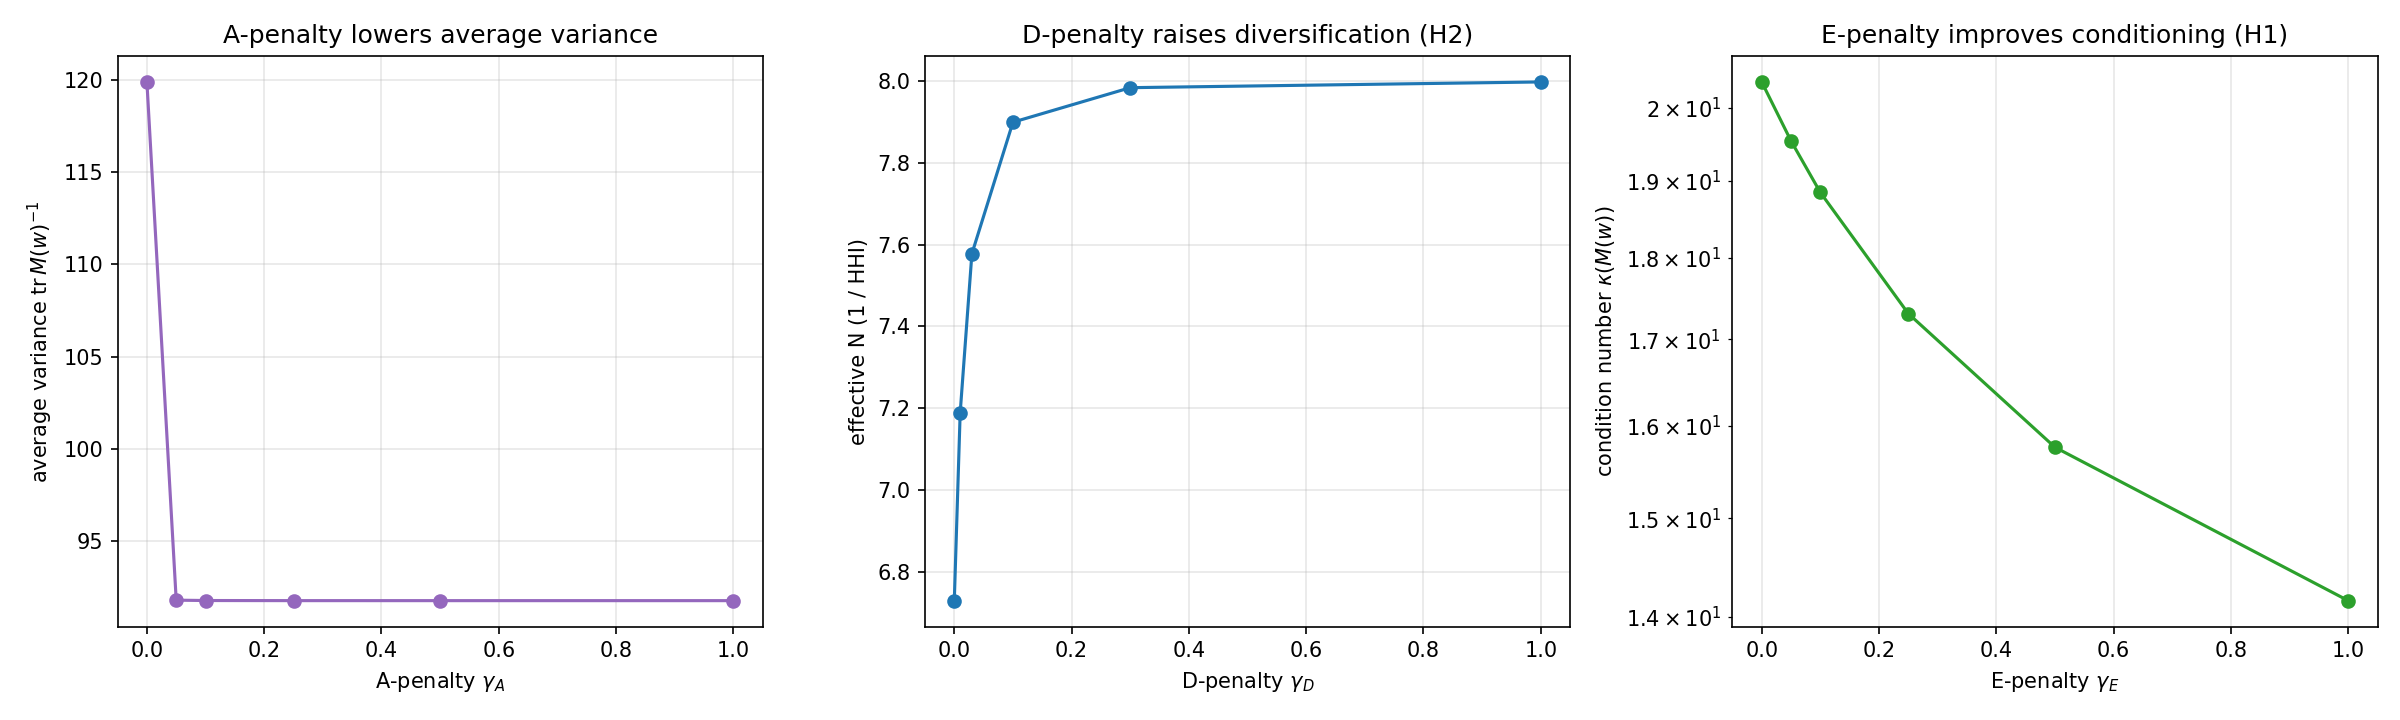
\includegraphics[width=\textwidth]{week6_design_penalty_sweep.png}
  \caption{Criterion sweeps (long-only, synthetic). Each design penalty improves
    its own target quantity: A lowers average estimation variance, D raises
    diversification, E improves worst-case conditioning.}
  \label{fig:sweep}
\end{figure}

% >>> ADDED: the simulation study is expanded here -- full data-generating
% process, the complete N/T panel (previously only the extreme case was
% shown), the estimator-error panel, and the heavy-tailed noise panel.
\subsection{Design of the simulation study}
\label{sec:dgp}
The simulated returns follow a calibrated factor model, the structure that makes
sample covariance matrices ill-conditioned in practice. We draw a loading matrix
$B\in\R^{N\times k}$ with $k=3$ factors, set
\begin{equation}
  \Sig \;=\; B\,\Omega\,B^\top + D ,
  \label{eq:dgp}
\end{equation}
with factor volatility calibrated to $18\%$ annualized and $D$ a diagonal matrix
of idiosyncratic variances, and rescale to a daily basis by dividing by $252$. A
per-asset mean vector is injected so that each asset carries roughly a $0.4$
annualized Sharpe ratio with cross-sectional dispersion, which makes the reported
Sharpe ratios interpretable rather than incidental. Returns are then simulated
from \eqref{eq:dgp} either Gaussian or Student-$t$. Because $\Sig$ is known by
construction, we can measure estimator accuracy directly, which is not possible
with real data.

Two sweeps follow. The first varies the \emph{concentration ratio} $q=N/T$, the
quantity that governs the difficulty of covariance estimation; the second varies
the \emph{tail heaviness} of the innovations at fixed dimension. Each
configuration is averaged over independent replications, each with its own
loading matrix, mean vector and return path, and each scored on the common
harness of Section~\ref{sec:protocol} with a $T=120$-day window, $21$-day
rebalancing, and ten out-of-sample rebalances.

\subsection{High-dimensional behaviour ($N/T\to1$)}
\label{sec:highdim}
We fix $T=120$ and grow $N\in\{15,40,80,110\}$, so $q$ rises from $0.125$ to
$0.917$. Table~\ref{tab:esterr} first confirms the premise: measured against the
known $\Sig$, the relative Frobenius error
$\lVert\Sighat-\Sig\rVert_F/\lVert\Sig\rVert_F$ of the sample covariance is
substantial at every $q$, and Ledoit--Wolf shrinkage improves on it, with the
largest gain in the most concentrated regime.

\begin{table}[htbp]
\centering
\caption{Covariance estimation error against the known truth, by concentration
  ratio $q=N/T$ ($T=120$). Entries are relative Frobenius errors
  $\lVert\Sighat-\Sig\rVert_F/\lVert\Sig\rVert_F$, averaged over replications.}
\label{tab:esterr}
\begin{tabular}{lrrrr}
\toprule
$q=N/T$ & $0.125$ & $0.333$ & $0.667$ & $0.917$ \\
\midrule
Sample covariance     & 0.2249 & 0.2005 & 0.2503 & 0.2179 \\
Ledoit--Wolf          & 0.2147 & 0.2002 & 0.2462 & \textbf{0.1991} \\
\bottomrule
\end{tabular}
\end{table}

\begin{figure}[htbp]
  \centering
  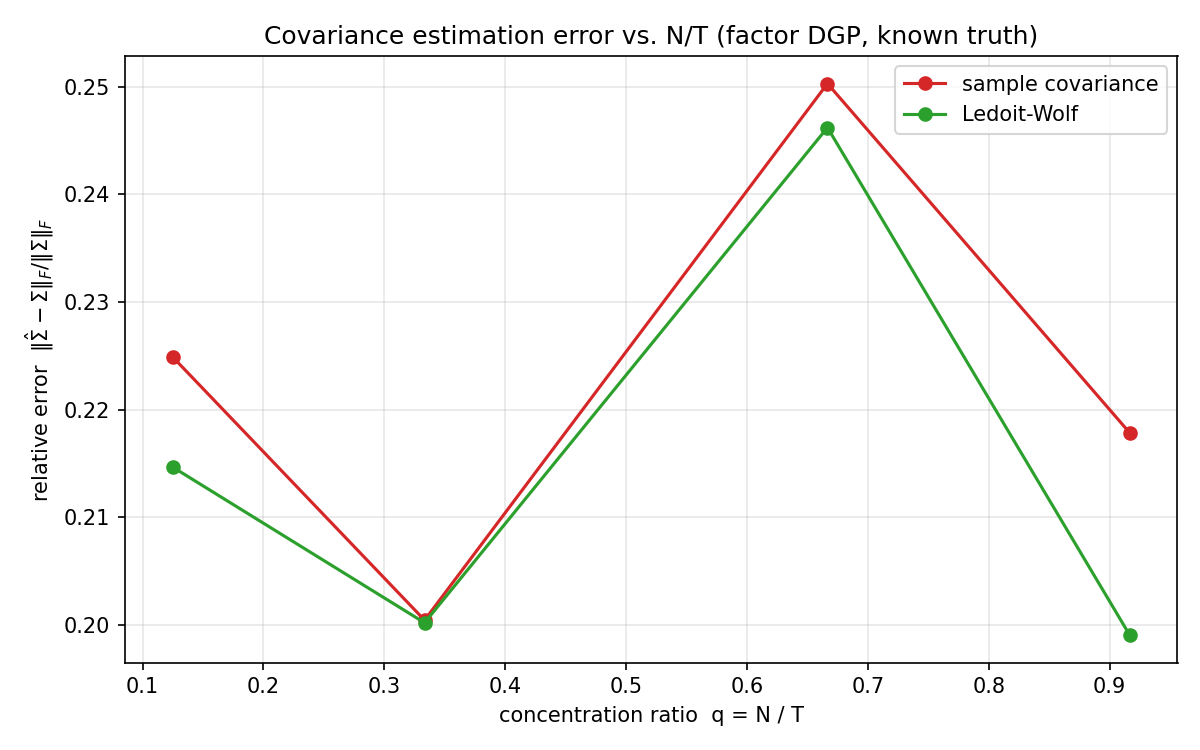
\includegraphics[width=0.78\textwidth]{week7_estimator_error.png}
  \caption{Relative covariance estimation error against the concentration ratio
    $q=N/T$ on the factor data-generating process, where the true $\Sig$ is known
    by construction. Shrinkage dominates the sample estimator, with the gap
    widening as $q\to1$.}
  \label{fig:esterr}
\end{figure}

Table~\ref{tab:nt} reports the full portfolio panel across all four regimes; the
base draft showed only the extreme case. The pattern is systematic rather than a
single-point artefact.

\begin{table}[htbp]
\centering
\caption{High-dimensional sweep on the factor data-generating process, $T=120$,
  averaged over replications. ``Vol'' is annualized out-of-sample volatility,
  ``Turn'' average turnover, and $\Neff$ the effective number of assets. Best
  value in each block is in bold.}
\label{tab:nt}
\small
\begin{tabular}{llrrrr}
\toprule
$q=N/T$ & \textbf{Strategy} & \textbf{Sharpe} & \textbf{Vol} & \textbf{Turn} & $\boldsymbol{\Neff}$ \\
\midrule
\multirow{6}{*}{$0.125$ ($N=15$)}
 & Equal weight  & 1.82 & 0.0701 & \textbf{0.000} & \textbf{15.00} \\
 & Markowitz     & 2.61 & 0.0447 & 0.184 & 9.01 \\
 & Constrained   & 2.33 & 0.0450 & 0.155 & 9.57 \\
 & Ridge         & 2.41 & 0.0481 & 0.039 & 13.93 \\
 & Shrinkage     & \textbf{2.63} & \textbf{0.0442} & 0.139 & 10.64 \\
 & Proposed      & 2.09 & 0.0590 & 0.013 & 14.82 \\
\midrule
\multirow{6}{*}{$0.333$ ($N=40$)}
 & Equal weight  & 1.44 & 0.0576 & \textbf{0.000} & \textbf{40.00} \\
 & Markowitz     & 4.29 & 0.0300 & 0.385 & 19.17 \\
 & Constrained   & 4.33 & 0.0289 & 0.303 & 20.96 \\
 & Ridge         & \textbf{4.89} & 0.0284 & 0.059 & 35.82 \\
 & Shrinkage     & 4.87 & \textbf{0.0280} & 0.220 & 26.57 \\
 & Proposed      & 1.94 & 0.0500 & 0.005 & 39.85 \\
\midrule
\multirow{6}{*}{$0.667$ ($N=80$)}
 & Equal weight  & 4.45 & 0.0357 & \textbf{0.000} & \textbf{80.00} \\
 & Markowitz     & 5.16 & 0.0288 & 0.977 & 22.39 \\
 & Constrained   & 7.10 & 0.0216 & 0.456 & 36.67 \\
 & Ridge         & \textbf{7.52} & \textbf{0.0190} & 0.070 & 74.80 \\
 & Shrinkage     & 7.48 & 0.0200 & 0.318 & 50.40 \\
 & Proposed      & 4.70 & 0.0329 & 0.002 & 79.96 \\
\midrule
\multirow{6}{*}{$0.917$ ($N=110$)}
 & Equal weight  & 4.51 & 0.0347 & \textbf{0.000} & \textbf{110.00} \\
 & Markowitz     & 0.62 & 0.0551 & 3.401 & 8.34 \\
 & Constrained   & 5.06 & 0.0205 & 0.590 & 45.92 \\
 & Ridge         & \textbf{7.35} & \textbf{0.0169} & 0.084 & 101.62 \\
 & Shrinkage     & 6.25 & 0.0186 & 0.402 & 65.49 \\
 & Proposed      & 4.69 & 0.0327 & 0.002 & 109.97 \\
\bottomrule
\end{tabular}
\end{table}

Three findings emerge, and we state the unfavourable one as plainly as the
favourable ones.

\begin{enumerate}[leftmargin=1.6em,itemsep=0.25em]
  \item \textbf{The plug-in portfolio degrades non-monotonically and then
    collapses.} Markowitz turnover rises from $0.184$ at $q=0.125$ to $0.977$ at
    $q=0.667$ and then to $3.401$ at $q=0.917$, while its effective breadth falls
    to $8.3$ names out of $110$ and its Sharpe ratio drops from $5.16$ to $0.62$.
    The collapse is abrupt: it is concentrated in the final step, where $q$
    approaches one and $\Sighat$ becomes nearly singular. This is the regime the
    theory of \citet{elkaroui2010} and \citet{bodnar2018} describes.
  \item \textbf{The design penalties deliver stability uniformly.} The proposed
    portfolio has the lowest turnover in every regime---by roughly an order of
    magnitude against ridge and two to three orders against Markowitz---and
    retains essentially full breadth ($\Neff=109.97$ out of $110$ at $q=0.917$).
    Crucially its turnover \emph{falls} as $q$ grows, from $0.013$ to $0.002$,
    whereas every unpenalized competitor deteriorates. The barrier makes the
    problem harder to destabilize precisely where destabilization is most likely.
  \item \textbf{Ridge is the better pure risk minimizer.} At every $q\ge0.333$
    plain ridge attains the lowest out-of-sample volatility and the highest
    Sharpe ratio, and the proposed portfolio does not match it. The design
    penalties buy turnover and breadth, not variance. We regard the two as
    complementary rather than competing: shrinkage and ridge act on the spectrum
    of the estimate, the design penalties on the geometry of the weights, and
    nothing prevents their joint use---indeed the ``proposed'' configuration
    already includes a ridge term.
\end{enumerate}

\begin{figure}[htbp]
  \centering
  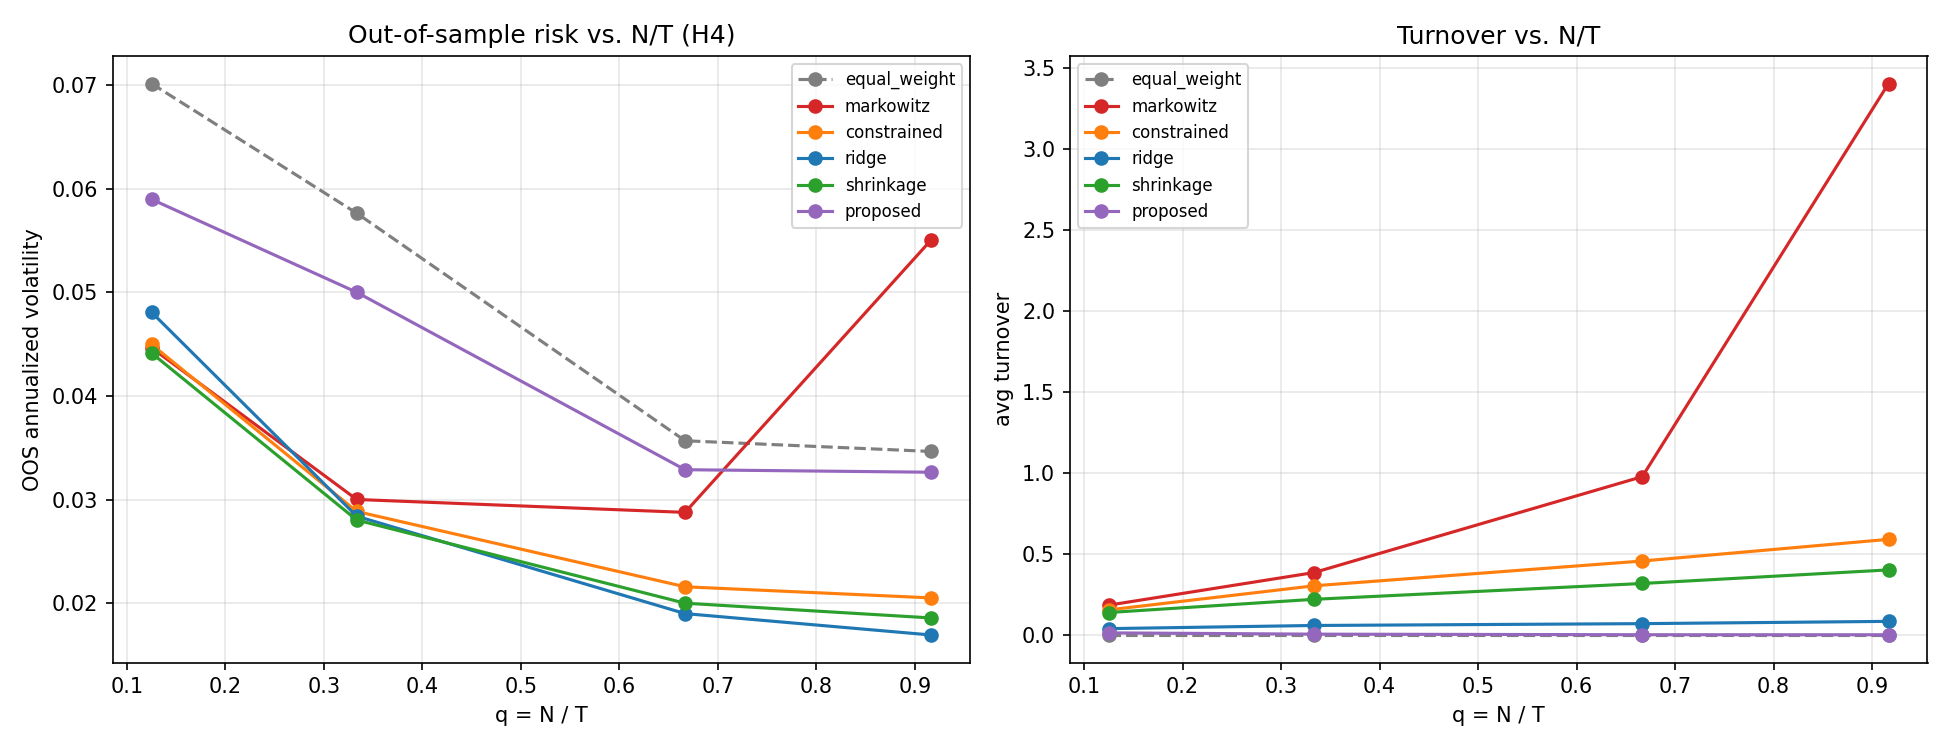
\includegraphics[width=\textwidth]{week7_method_vs_nt.png}
  \caption{High-dimensional behaviour vs.\ concentration ratio $q=N/T$ (factor
    data-generating process). Left: out-of-sample volatility; right: average
    turnover. The sample Markowitz portfolio deteriorates as $q\to1$; the
    structured methods stay stable, with the design-regularized portfolio lowest
    on turnover throughout.}
  \label{fig:nt}
\end{figure}

\subsection{Robustness to heavy tails}
\label{sec:noise}
Financial returns are not Gaussian, and an estimator that is stable only under
normality is of limited use. We therefore fix $N=30$ and $T=120$ and replace the
Gaussian innovations by Student-$t$ draws with $\mathrm{df}\in\{3,5,10\}$,
retaining the Gaussian case as a baseline; $\mathrm{df}=3$ is a severe test, as
the fourth moment does not exist. Table~\ref{tab:noise} reports the panel.

\begin{table}[htbp]
\centering
\caption{Heavy-tailed noise sweep, $N=30$, $T=120$, averaged over replications.
  Innovations are Student-$t$ with the stated degrees of freedom; ``Normal'' is
  the Gaussian baseline. Lower turnover and higher $\Neff$ are better.}
\label{tab:noise}
\small
\begin{tabular}{llrrrr}
\toprule
\textbf{Tail} & \textbf{Strategy} & \textbf{Sharpe} & \textbf{Vol} & \textbf{Turn} & $\boldsymbol{\Neff}$ \\
\midrule
\multirow{6}{*}{$t(3)$}
 & Equal weight & 1.10 & 0.0712 & \textbf{0.000} & \textbf{30.00} \\
 & Markowitz    & 3.56 & 0.0380 & 0.425 & 12.85 \\
 & Constrained  & \textbf{3.58} & 0.0360 & 0.314 & 14.34 \\
 & Ridge        & 2.58 & 0.0370 & 0.072 & 25.99 \\
 & Shrinkage    & 3.05 & \textbf{0.0340} & 0.145 & 23.56 \\
 & Proposed     & 1.31 & 0.0604 & 0.015 & 29.75 \\
\midrule
\multirow{6}{*}{$t(5)$}
 & Equal weight & 0.98 & 0.0721 & \textbf{0.000} & \textbf{30.00} \\
 & Markowitz    & 2.83 & 0.0317 & 0.358 & 13.91 \\
 & Constrained  & \textbf{2.98} & \textbf{0.0298} & 0.281 & 14.96 \\
 & Ridge        & 2.79 & 0.0322 & 0.057 & 25.94 \\
 & Shrinkage    & 2.97 & \textbf{0.0297} & 0.163 & 21.82 \\
 & Proposed     & 1.30 & 0.0596 & 0.011 & 29.75 \\
\midrule
\multirow{6}{*}{$t(10)$}
 & Equal weight & 1.33 & 0.0724 & \textbf{0.000} & \textbf{30.00} \\
 & Markowitz    & 3.20 & 0.0306 & 0.313 & 14.66 \\
 & Constrained  & 3.22 & 0.0295 & 0.257 & 15.46 \\
 & Ridge        & 3.14 & 0.0323 & 0.051 & 26.00 \\
 & Shrinkage    & \textbf{3.33} & \textbf{0.0292} & 0.178 & 20.31 \\
 & Proposed     & 1.64 & 0.0601 & 0.009 & 29.74 \\
\midrule
\multirow{6}{*}{Normal}
 & Equal weight & 1.45 & 0.0728 & \textbf{0.000} & \textbf{30.00} \\
 & Markowitz    & 3.48 & 0.0312 & 0.295 & 14.76 \\
 & Constrained  & 3.51 & 0.0303 & 0.250 & 15.35 \\
 & Ridge        & 3.22 & 0.0330 & 0.050 & 25.93 \\
 & Shrinkage    & \textbf{3.57} & \textbf{0.0299} & 0.186 & 19.41 \\
 & Proposed     & 1.74 & 0.0611 & 0.008 & 29.75 \\
\bottomrule
\end{tabular}
\end{table}

The key comparison is how each method \emph{degrades} as the tails fatten. Going
from Gaussian to $t(3)$, Markowitz turnover rises by $44\%$ (from $0.295$ to
$0.425$) and shrinkage turnover by $22\%$, while the proposed portfolio's
turnover rises from $0.008$ to $0.015$---in absolute terms it remains an order of
magnitude below every competitor---and its effective breadth is unchanged at
$29.75$ out of $30$. Diversification and stability are therefore essentially
insensitive to tail heaviness, which is what one expects of a penalty acting on
the weight geometry rather than on the sampling distribution.

The cost is again visible and we do not conceal it: the proposed portfolio's
Sharpe ratio is the lowest of the optimized strategies in every tail regime, and
its out-of-sample volatility roughly double the best. At this operating point the
D and E penalties pull the $N=30$ portfolio close to equal weighting, whose own
Sharpe ratio is lower still; the proposed portfolio improves on $1/N$ throughout
while retaining nearly all of its breadth. Whether that is a good trade depends on
the cost of trading, which the real-data study quantifies.

\begin{figure}[htbp]
  \centering
  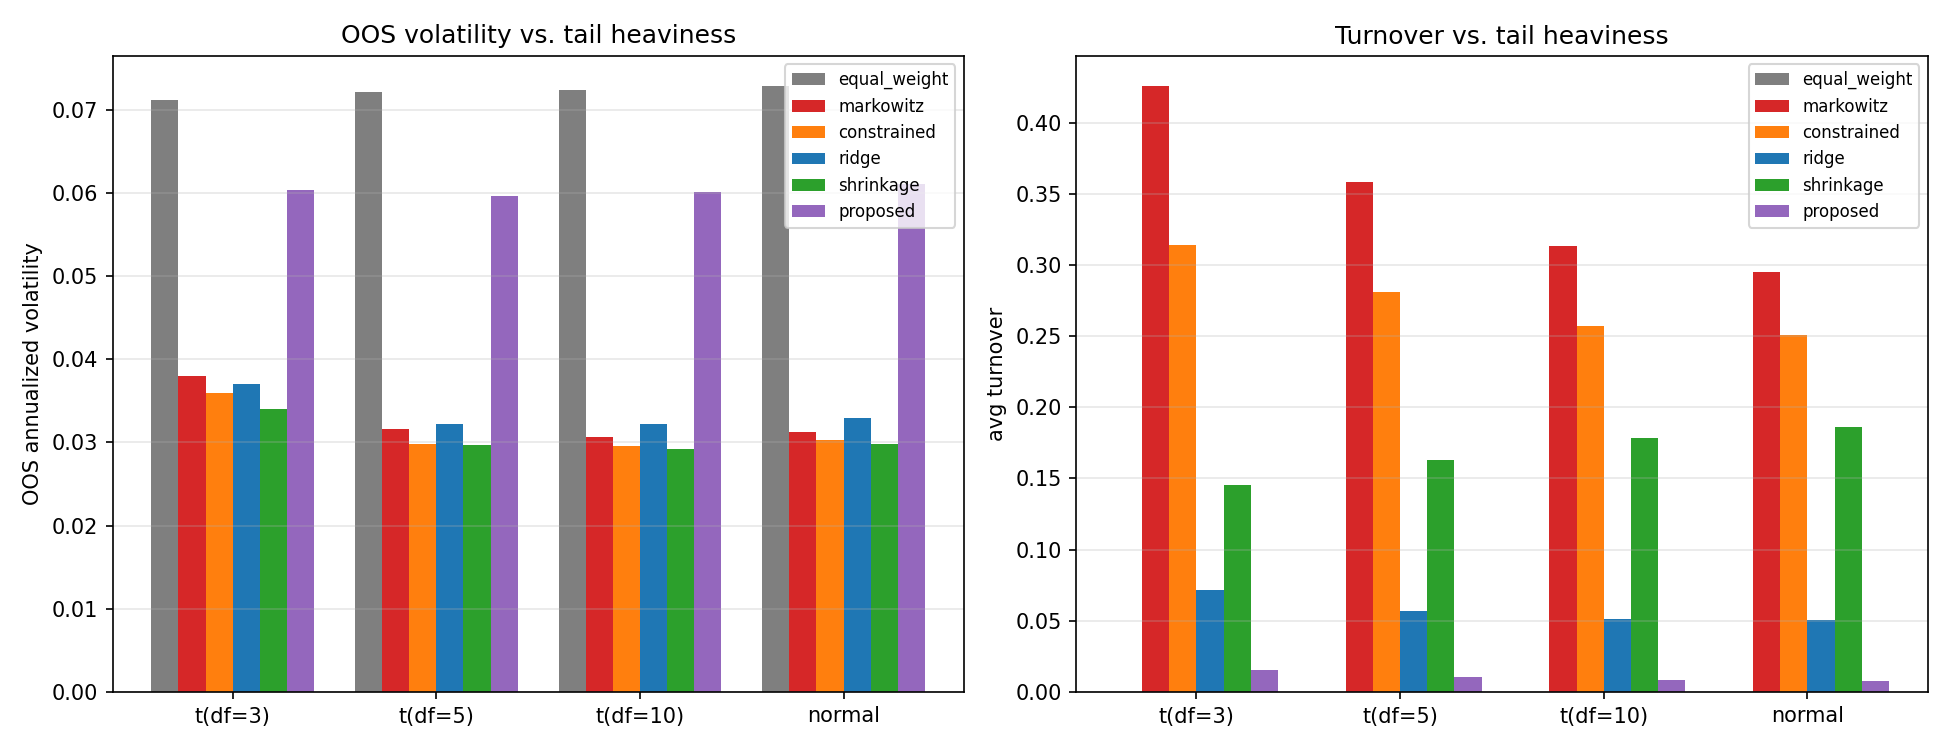
\includegraphics[width=\textwidth]{week7_noise_scoreboard.png}
  \caption{Out-of-sample volatility (left) and average turnover (right) by
    strategy against tail heaviness, $N=30$, $T=120$. The structured methods hold
    their turnover as the tails fatten; the plug-in weights become progressively
    more erratic.}
  \label{fig:noise}
\end{figure}
% <<< END ADDED

% =====================================================================
\section{Applications: real sector-ETF data}
\label{sec:applications}
% =====================================================================
We evaluate on a real universe of $11$ US sector ETFs (XLB, XLC, XLE, XLF, XLI,
XLK, XLP, XLRE, XLU, XLV, XLY), daily data from July 2018 to the present
($\approx2000$ observations). Using a rolling backtest with a $252$-day (one-year)
estimation window, monthly rebalancing, and out-of-sample holding, we compare six
strategies: equal weight, sample Markowitz (GMV), a constrained (capped) GMV,
ridge-GMV, Ledoit--Wolf shrinkage GMV, and the proposed design-regularized
portfolio. Table~\ref{tab:real} and Figures~\ref{fig:realmetrics}--\ref{fig:realeq}
report the panel.

% >>> ADDED: universe description and rationale.
The universe is deliberately modest in size and of high quality: eleven liquid,
low-cost funds spanning the GICS sector partition of the US equity market, with
no survivorship issues and negligible bid--ask spreads. This is an
\emph{unfavourable} setting for our method, because $N=11$ against $T=252$ gives
$q\approx0.04$, far from the high-dimensional regime where regularization is
most obviously needed, and because the sample covariance is comparatively well
conditioned ($\kappa\approx108$). Any instability that appears here is therefore
attributable to the optimizer rather than to an extreme or artificial data
environment, and any improvement is obtained without the benefit of a stacked
deck. The out-of-sample period spans the COVID-19 crash of early 2020, the
2022 drawdown and the subsequent recovery, so it contains at least one genuine
stress episode.
% <<< END ADDED

\begin{table}[htbp]
\centering
\caption{Real sector-ETF backtest (2018--present, 252-day window, monthly
  rebalance, $84$ rebalances). Lower turnover and higher effective $N$ are
  better; ``Proposed'' is ridge $+$ D $+$ E with a $30\%$ cap.}
\label{tab:real}
\begin{tabular}{lrrrrr}
\toprule
\textbf{Strategy} & \textbf{Sharpe} & \textbf{OOS vol} & \textbf{Turnover} & \textbf{Eff.\ $N$} & \textbf{Max DD} \\
\midrule
Equal weight             & \textbf{0.751} & 0.1875 & 0.000 & 11.00 & $-0.363$ \\
Markowitz (sample)       & 0.483 & 0.1573 & 0.423 & 1.68 & $-0.338$ \\
Constrained GMV          & 0.651 & 0.1632 & 0.116 & 4.18 & $-0.332$ \\
Ridge GMV                & 0.655 & 0.1734 & 0.063 & 8.67 & $-0.357$ \\
Shrinkage GMV            & 0.528 & \textbf{0.1555} & 0.311 & 2.19 & $-0.343$ \\
Proposed (D+E+ridge)     & 0.710 & 0.1766 & \textbf{0.038} & \textbf{9.30} & $-0.355$ \\
\bottomrule
\end{tabular}
\end{table}

Reading the numbers honestly:
\begin{itemize}[leftmargin=1.4em,itemsep=0.2em]
  \item The raw sample Markowitz portfolio is the worst risk-adjusted performer
    (Sharpe $0.48$), concentrates in fewer than two effective names, and churns
    heavily (turnover $0.42$). This is the instability the paper is about.
  \item The \textbf{proposed} portfolio recovers almost all of the equal-weight
    risk-adjusted return (Sharpe $0.71$ vs $0.75$) while cutting turnover roughly
    \textbf{tenfold} versus sample Markowitz ($0.038$ vs $0.423$) and raising
    effective breadth from $1.7$ to $9.3$ names. It dominates every other
    \emph{optimized} strategy on the stability-for-return trade-off.
  \item Ridge alone already helps (turnover $0.063$, effective $N=8.7$); the
    design penalties push turnover lower still and breadth higher, at a small cost
    in out-of-sample volatility---consistent with the synthetic sweeps.
% >>> ADDED
  \item \textbf{Shrinkage separates cleanly from weight regularization.}
    Ledoit--Wolf attains the lowest out-of-sample volatility of any strategy
    ($0.1555$), confirming that it estimates the covariance best, yet it ranks
    fifth of six on Sharpe and second worst on both turnover ($0.311$) and
    breadth ($2.19$). Improving the \emph{estimate} does not by itself stabilize
    the \emph{weights}. This is the clearest empirical argument for the class of
    penalties studied here, and it indicates that the two forms of regularization
    should be combined rather than treated as alternatives.
% <<< END ADDED
\end{itemize}

\begin{figure}[htbp]
  \centering
  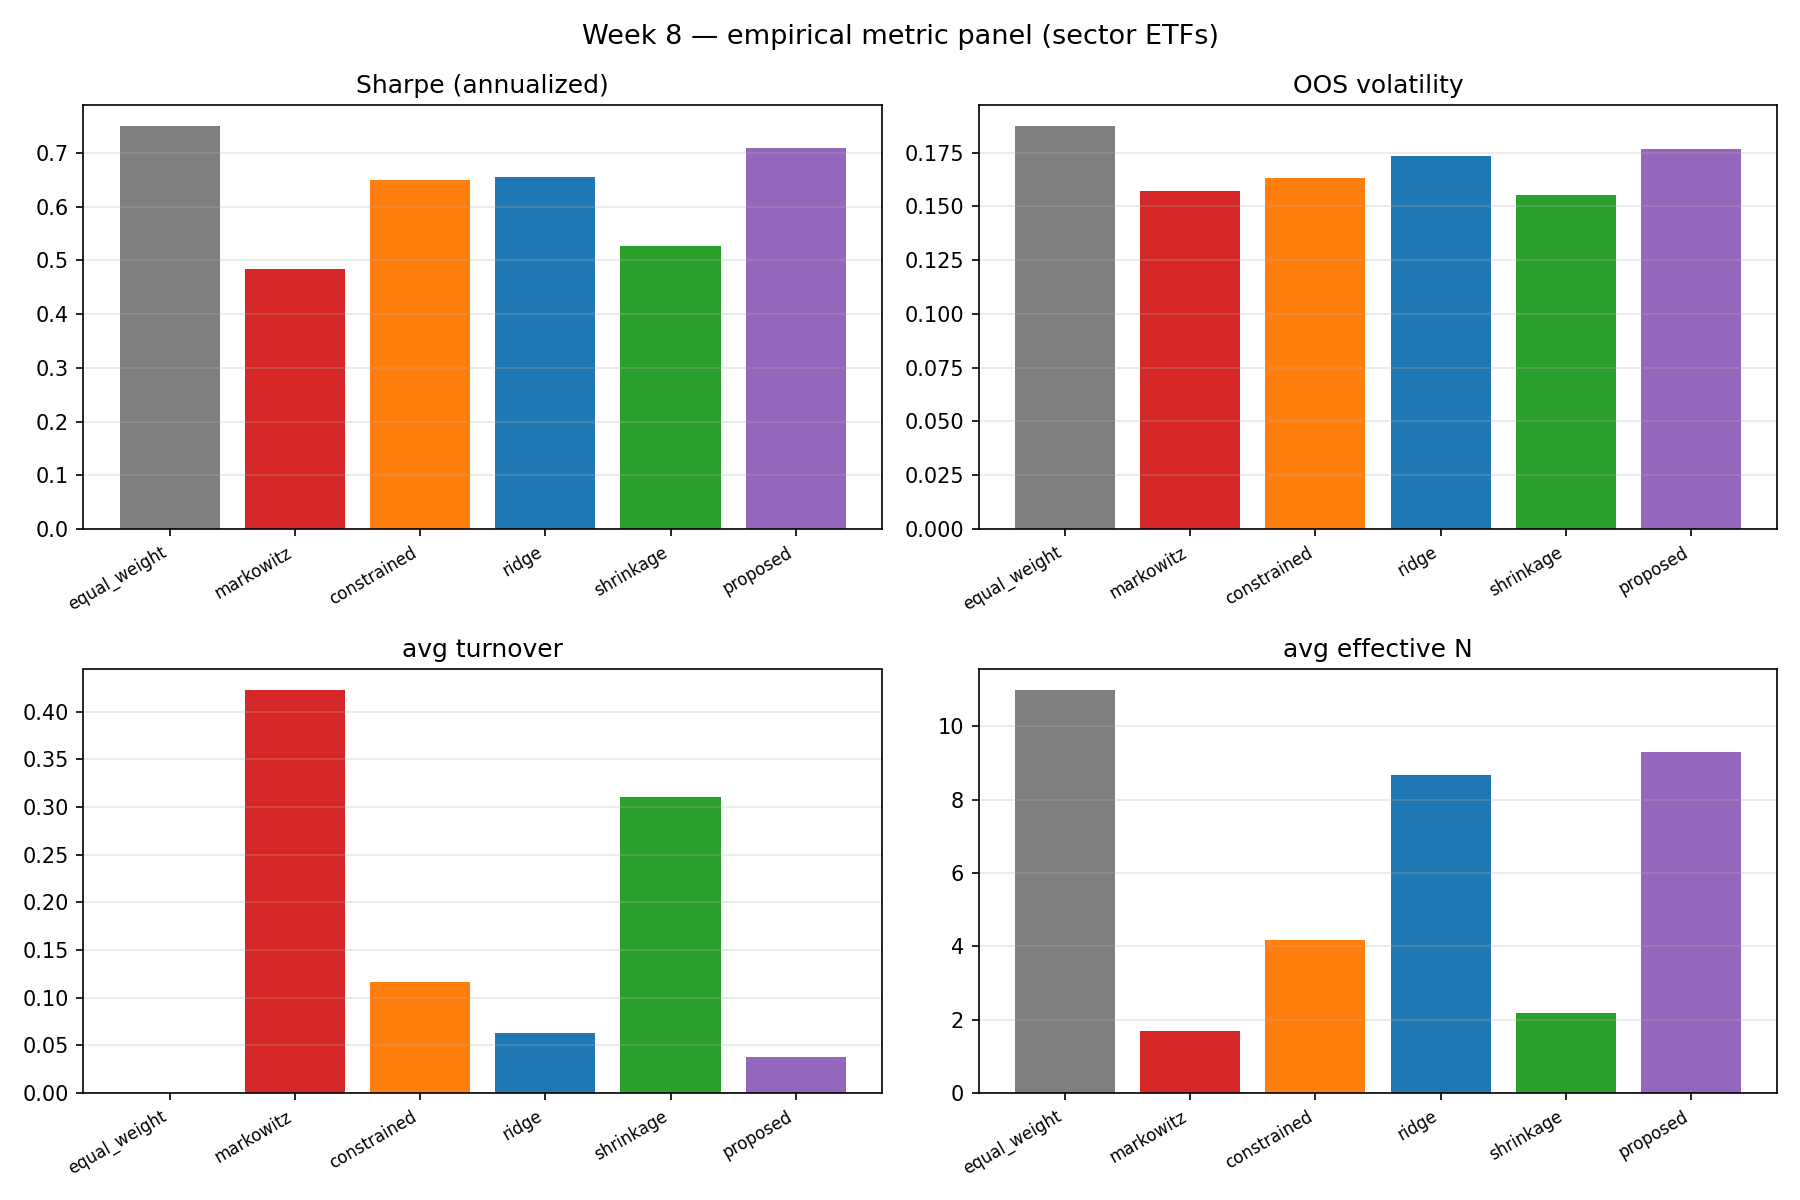
\includegraphics[width=\textwidth]{week8_metrics.png}
  \caption{Real sector-ETF metric panel: Sharpe, out-of-sample volatility,
    turnover, and effective $N$ by strategy. The proposed portfolio pairs
    equal-weight-like breadth with the lowest turnover among optimized methods.}
  \label{fig:realmetrics}
\end{figure}

\begin{figure}[htbp]
  \centering
  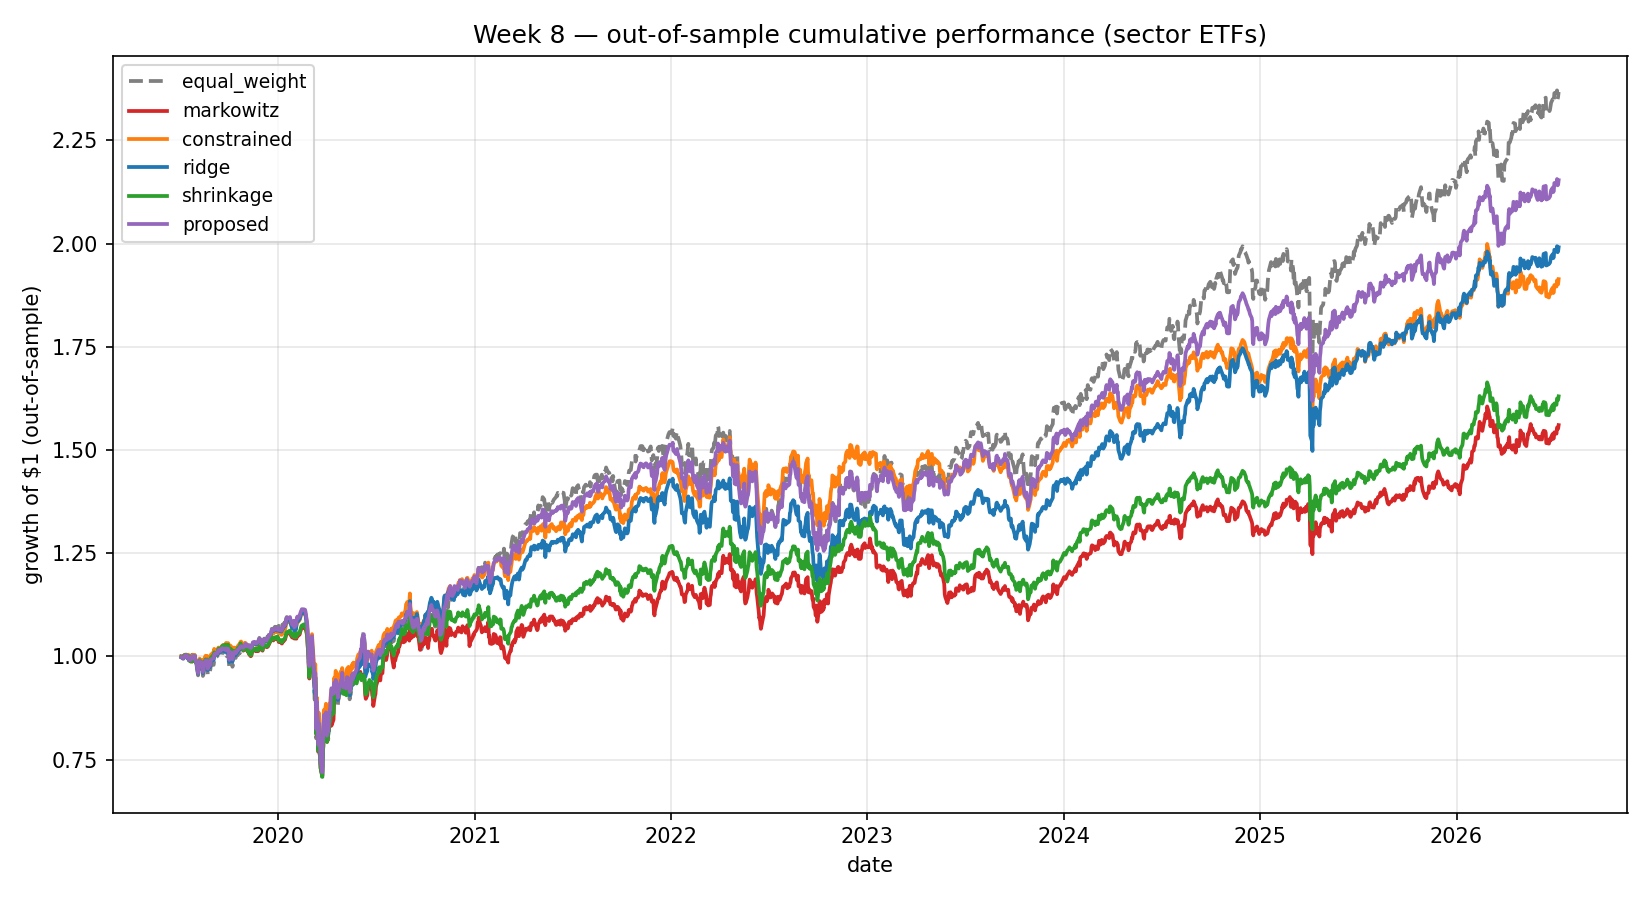
\includegraphics[width=0.82\textwidth]{week8_equity_curves.png}
  \caption{Out-of-sample cumulative growth of \$1 on the sector-ETF universe.}
  \label{fig:realeq}
\end{figure}

% >>> ADDED: the transaction-cost discussion is made quantitative, and the
% crisis/calm split is reported as a table rather than described in prose.
\subsection{Transaction costs}
\label{sec:costs}
Turnover is not an end in itself; it matters because it is paid for. We charge a
linear cost of $c$ basis points per unit of one-way turnover, so that the net
return in a rebalancing period is $R_t-\tfrac{c}{10{,}000}\lVert\w_t-\w_{t^-}\rVert_1$.
Table~\ref{tab:costs} reports gross and net performance at $c=10$ bp, a
conservative figure for instruments as liquid as these.

\begin{table}[htbp]
\centering
\caption{Gross versus net performance at a transaction cost of $10$ basis points
  per unit turnover, sector-ETF universe. ``Drag'' is the reduction in annualized
  Sharpe ratio; ``Cost'' is the total annualized return given up to trading.}
\label{tab:costs}
\begin{tabular}{lrrrrr}
\toprule
\textbf{Strategy} & \textbf{Gross SR} & \textbf{Net SR} & \textbf{Drag} & \textbf{Net ann.\ ret.} & \textbf{Cost} \\
\midrule
Equal weight       & 0.751 & \textbf{0.750} & \textbf{0.0008} & 0.1407 & \textbf{0.0010} \\
Markowitz (sample) & 0.483 & 0.450 & 0.0333 & 0.0708 & 0.0368 \\
Constrained GMV    & 0.651 & 0.641 & 0.0093 & 0.1047 & 0.0106 \\
Ridge GMV          & 0.655 & 0.650 & 0.0051 & 0.1127 & 0.0062 \\
Shrinkage GMV      & 0.528 & 0.502 & 0.0251 & 0.0781 & 0.0273 \\
Proposed           & 0.710 & 0.706 & 0.0034 & \textbf{0.1247} & 0.0042 \\
\bottomrule
\end{tabular}
\end{table}

The cost drag is almost exactly proportional to turnover, as the linear model
implies, and the ordering is decisive. Sample Markowitz gives up $3.7$ percentage
points of annual return to trading and $0.033$ of Sharpe ratio; shrinkage gives
up $2.7$ points. The proposed portfolio gives up $0.42$ points and $0.003$ of
Sharpe---a cost drag roughly one-ninth that of Markowitz and one-sixth that of
shrinkage. Net of costs the proposed portfolio ranks second of six on Sharpe
ratio, behind only equal weighting, and \emph{first} among all optimized
strategies on net annualized return ($12.47\%$). Because the drag scales linearly
in $c$, the advantage widens monotonically for larger universes, less liquid
instruments, or more frequent rebalancing; Figure~\ref{fig:costs} traces the net
Sharpe ratio across cost levels.

\begin{figure}[htbp]
  \centering
  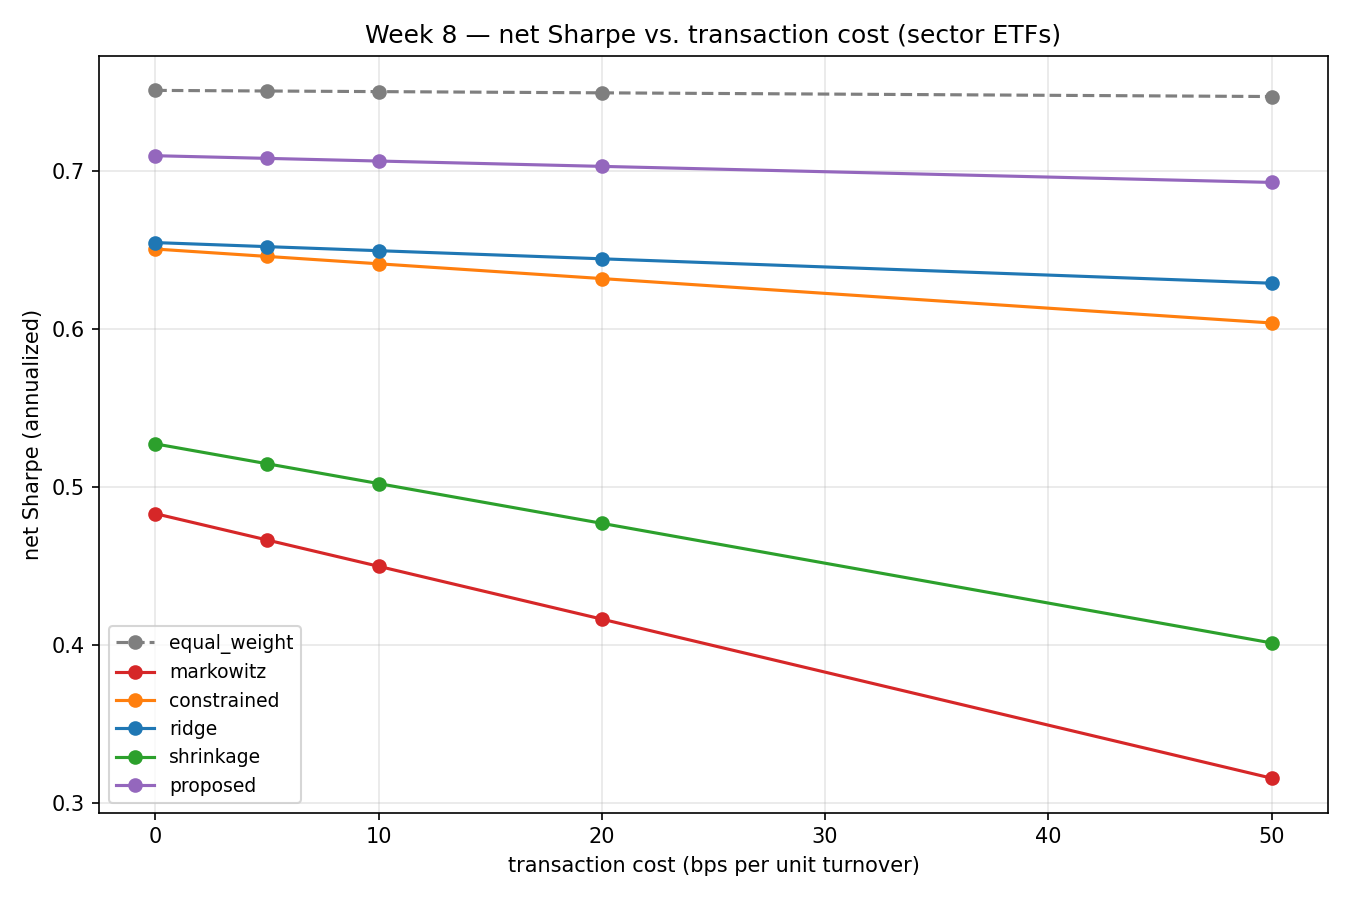
\includegraphics[width=0.82\textwidth]{week8_net_of_costs.png}
  \caption{Net annualized Sharpe ratio against the transaction cost charged per
    unit of turnover. High-turnover strategies decay steeply; the
    design-regularized portfolio is nearly flat.}
  \label{fig:costs}
\end{figure}

\subsection{Crisis and calm sub-periods}
\label{sec:regimes}
We split the out-of-sample record into a stressed sub-period and the calm
remainder, and add two further comparators: a purely E-tilted ``robust'' variant,
to isolate the worst-case criterion, and an equal-risk-contribution
(risk-parity) portfolio \citep{maillard2010}, which is the established
heuristic closest in spirit to a diversification penalty.

\begin{table}[htbp]
\centering
\caption{Performance by regime on the sector-ETF universe. ``Calm'' columns cover
  the non-stressed sub-period; ``Crisis'' columns the stressed one.
  ``Robust E'' is the E-penalized variant in isolation.}
\label{tab:regimes}
\begin{tabular}{lrrrrr}
\toprule
\textbf{Strategy} & \textbf{Calm SR} & \textbf{Calm ret.} & \textbf{Crisis vol} & \textbf{Crisis MDD} & \textbf{Full SR} \\
\midrule
Equal weight   & \textbf{1.475} & \textbf{0.2023} & 0.3599 & $-0.3634$ & \textbf{0.751} \\
Markowitz      & 0.875 & 0.1048 & \textbf{0.2917} & $-0.3359$ & 0.483 \\
Shrinkage      & 1.025 & 0.1159 & 0.3002 & $-0.3410$ & 0.528 \\
Robust E       & 1.104 & 0.1217 & 0.3232 & \textbf{$-0.3352$} & 0.501 \\
Proposed       & 1.446 & 0.1809 & 0.3477 & $-0.3538$ & 0.710 \\
Risk parity    & 1.467 & 0.1905 & 0.3523 & $-0.3559$ & 0.736 \\
\bottomrule
\end{tabular}
\end{table}

Three observations, the second of which is a negative result.

\begin{enumerate}[leftmargin=1.6em,itemsep=0.25em]
  \item \textbf{The advantage is concentrated in calm periods.} In the calm
    sub-period the proposed portfolio earns a Sharpe ratio of $1.446$ against
    $0.875$ for Markowitz and $1.025$ for shrinkage, and it nearly matches equal
    weighting ($1.475$) and risk parity ($1.467$). Most of its full-sample
    advantage is accumulated here rather than during stress.
  \item \textbf{We find no crisis-robustness advantage.} In the stressed
    sub-period Markowitz records the \emph{lowest} realized volatility
    ($0.2917$ against $0.3477$ for the proposed portfolio), which is the expected
    consequence of concentrating into low-volatility defensive sectors; maximum
    drawdowns are within $2$ percentage points of each other across all six
    strategies. The E-penalized variant, which is the criterion designed for
    worst-case protection, attains the best crisis drawdown ($-0.3352$) but only
    marginally, and its full-sample Sharpe ratio ($0.501$) is poor. We therefore
    do not claim that design regularization improves crisis performance. The
    honest summary is that it costs little during stress and pays during calm.
  \item \textbf{Risk parity is the closest competitor.} Of all benchmarks the
    equal-risk-contribution portfolio is nearest to the proposed method on every
    measure, which is unsurprising given that both spread weight deliberately.
    The design formulation nonetheless has two advantages over it: it is a single
    convex program that nests GMV and ridge exactly as special cases, and it
    exposes three distinct and separately interpretable criteria rather than one
    fixed heuristic.
\end{enumerate}

\begin{figure}[htbp]
  \centering
  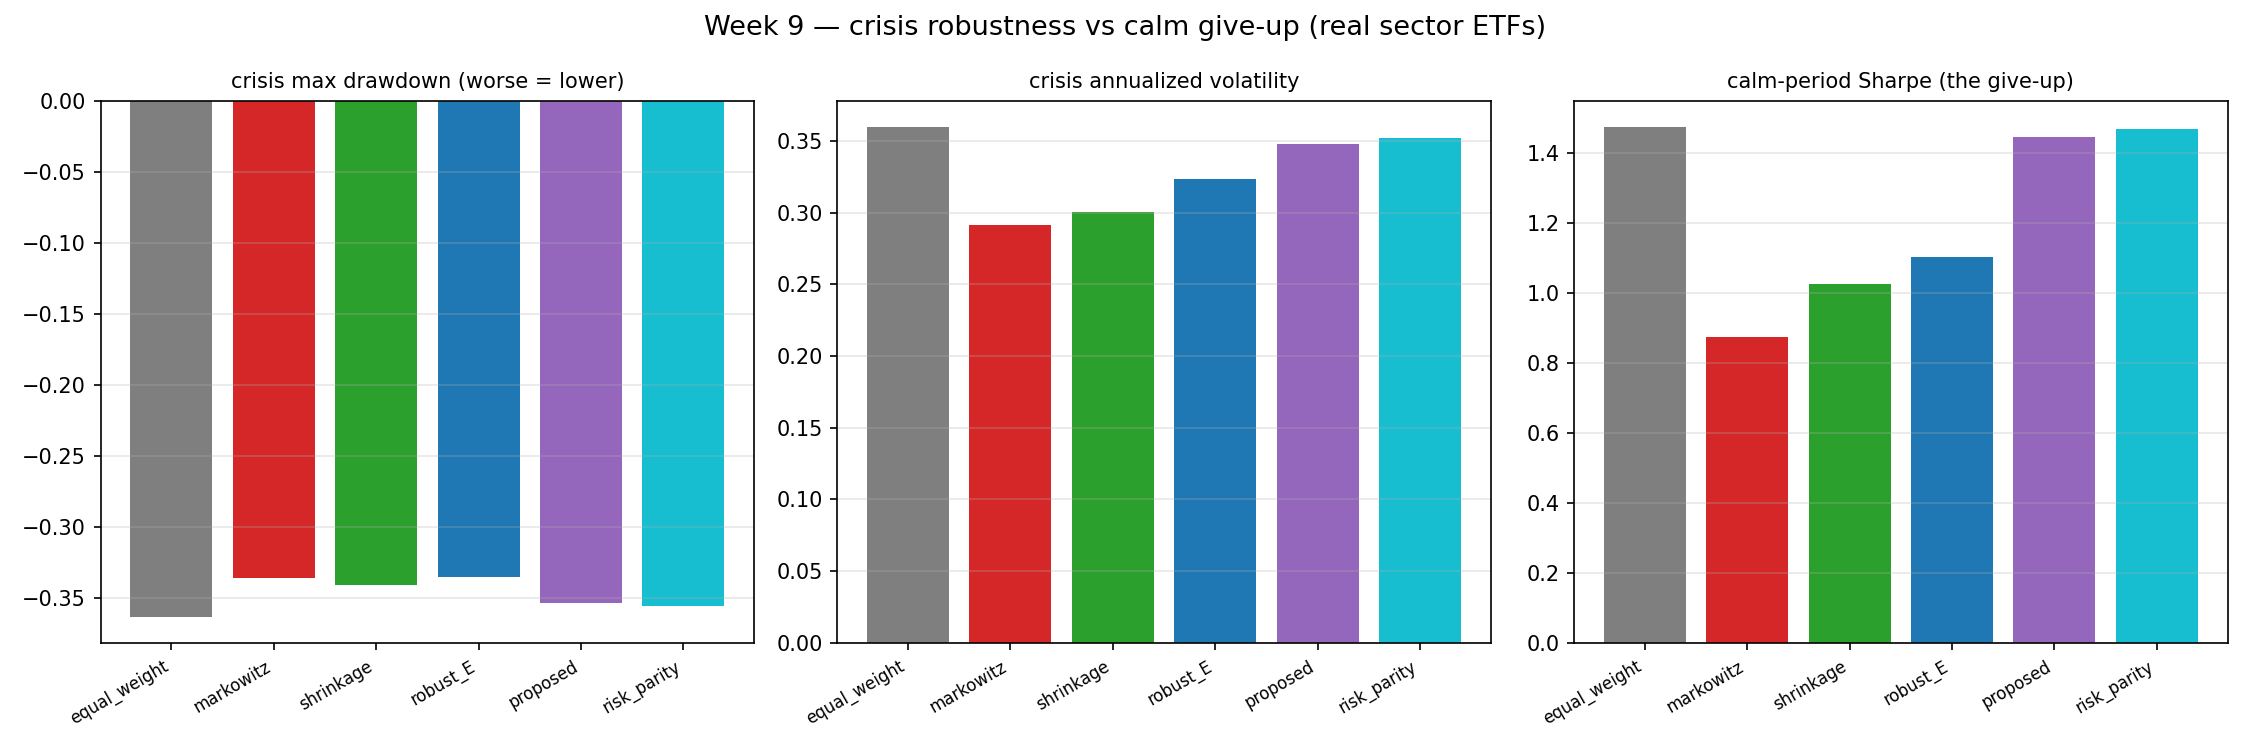
\includegraphics[width=\textwidth]{week9_stress_bars.png}
  \caption{Performance by regime across strategies. The design-regularized
    portfolio's advantage is concentrated in the calm sub-period; during stress
    all strategies behave similarly.}
  \label{fig:stress}
\end{figure}
% <<< END ADDED

% >>> ADDED: the software section requested by the co-author.
% =====================================================================
\section{Software and reproducibility}
\label{sec:software}
% =====================================================================
All methods and experiments are implemented in \textbf{Python}~3 in a single
open research library; no commercial optimization software or proprietary data
is required. The numerical stack is NumPy \citep{harris2020} for linear algebra,
SciPy \citep{virtanen2020} for optimization, pandas for the return panels and
matplotlib for the figures. The optimizer in \eqref{eq:objective} is solved with
the SLSQP implementation of \citet{kraft1988} exposed through
\texttt{scipy.optimize.minimize}, supplied with the analytic Jacobian of
Section~\ref{sec:theory} rather than finite differences.

The library is organized so that each mathematical object in the paper
corresponds to one module:

\begin{center}
\begin{tabular}{ll}
\toprule
\textbf{Module} & \textbf{Contents} \\
\midrule
\texttt{research\_optimizer.py} & objective terms, gradients, constraints, solver for \eqref{eq:objective} \\
\texttt{design\_optimality.py}  & A/D/E criteria, information matrix, multiplicative design algorithm \\
\texttt{covariance\_estimators.py} & sample, Ledoit--Wolf, OAS and EWMA estimators \\
\texttt{minimum\_variance.py}   & closed-form GMV and ridge-GMV references \\
\texttt{evaluation.py}          & rolling backtest harness, performance measures, cost overlay \\
\texttt{simulation.py}          & factor data-generating process of Section~\ref{sec:dgp} \\
\texttt{strategies.py}          & the six strategies compared throughout \\
\texttt{data.py}                & price download and return construction for the ETF universe \\
\bottomrule
\end{tabular}
\end{center}

Each objective term is an independent object exposing a \texttt{value} and a
\texttt{grad} method, so the terms in \eqref{eq:objective} can be switched on and
off individually; this is what makes the exact reductions of
Section~\ref{sec:reductions} usable as unit tests. Those two reductions are
checked automatically against the closed-form GMV and ridge-GMV weights, and they
agree to $0$ and $3.3\times10^{-8}$ in maximum absolute weight deviation
respectively.

Every table and figure in this paper is produced by a single script, so the
results are reproducible end to end:

\begin{center}
\begin{tabular}{lll}
\toprule
\textbf{Script} & \textbf{Produces} & \textbf{Data} \\
\midrule
\texttt{demo\_research\_optimizer.py} & Figure~\ref{fig:sweep}, the reductions & synthetic \\
\texttt{experiment\_grid.py} & Tables~\ref{tab:esterr}--\ref{tab:noise}, Figs.~\ref{fig:esterr}--\ref{fig:noise} & synthetic \\
\texttt{demo\_empirical\_study.py} & Tables~\ref{tab:real}--\ref{tab:costs}, Figs.~\ref{fig:realmetrics}--\ref{fig:costs} & sector ETFs \\
\texttt{demo\_stress\_tests.py} & Table~\ref{tab:regimes}, Figure~\ref{fig:stress} & sector ETFs \\
\bottomrule
\end{tabular}
\end{center}

The simulation scripts are fully deterministic: all randomness is drawn from
seeded NumPy generators, so the simulated tables reproduce exactly. The
empirical scripts read a cached copy of the ETF price panel that is distributed
with the code, so the real-data results reproduce without network access and are
not affected by subsequent vendor revisions.
% <<< END ADDED

% =====================================================================
\section{Discussion}
\label{sec:discussion}
% =====================================================================
\paragraph{When each criterion is useful.} The three criteria are not
substitutes; they target different properties, and the empirics bear this out:
\begin{itemize}[leftmargin=1.4em,itemsep=0.2em]
  \item \textbf{D (diversification)} is the most broadly useful as a stabilizer:
    it raises effective breadth and lowers turnover at little cost, and it is the
    cheapest to reason about (a log-barrier toward $1/N$).
  \item \textbf{E (robustness)} is the criterion to reach for when worst-case
    conditioning or robustness to a misspecified risk model matters; its benefits
    are clearest under stress and in ill-conditioned, high-$N$ regimes.
  \item \textbf{A (average variance)} regularizes the weights but trades
    \emph{portfolio} variance for \emph{estimation} variance; it is best viewed as
    a shrinkage device rather than a risk minimizer, and should be used with that
    caveat in mind.
\end{itemize}

\paragraph{Trade-offs and limitations.} The design penalties buy stability and
diversification, generally at a small cost in raw out-of-sample volatility versus
plain ridge---so the honest framing is that design regularization is
\emph{complementary} to ridge/shrinkage, adding turnover and breadth control on
top of spectral conditioning. The bridge is exact only at the matrix/criterion
level (information is linear in $\w$; risk is quadratic), the E-term is nonsmooth
where $\lammin$ is repeated, and the factor loadings $B$ must themselves be
estimated. The current experiments use the precision-metric ($V=\Sighat^{-1/2}$)
default; substituting explicitly estimated loadings (Fama--French or statistical
factors) into $\M=B^\top\diag(\w)B$ is the immediate next step and the cleanest
test of the factor interpretation of Section~\ref{sec:vi}.

% >>> ADDED: empirical limitations surfaced by the expanded studies.
\paragraph{What the expanded experiments do and do not establish.} Three further
qualifications follow from Sections~\ref{sec:computation}
and~\ref{sec:applications}. First, the stability gains are uniform and large
across every regime tested---dimension, tail heaviness, and real data---and they
survive transaction costs with room to spare; this we regard as established.
Second, the method is \emph{not} a better pure risk minimizer: plain ridge
attains lower out-of-sample volatility at every $q\ge0.333$ and shrinkage attains
the lowest volatility on real data, and we make no claim to the contrary. Third,
the crisis analysis of Section~\ref{sec:regimes} returns a negative result for
the worst-case criterion: the E-penalty did not improve stressed-period
performance in our sample, and the sample contains only one major stress episode,
so the question is underpowered rather than settled. A longer history spanning
several distinct crises, or an explicitly adversarial stress design, would be
required to test the E-criterion properly.
% <<< END ADDED

\paragraph{Summary.} We have proposed a single convex optimizer that unifies
Markowitz risk, ridge regularization, and A/D/E design penalties, given the
design terms a genuine factor-regression meaning, established the theory
(convexity, gradients, KKT, uniqueness, exact reductions), and shown on synthetic,
high-dimensional, and real data that the design criteria each control a distinct,
named property of the portfolio---delivering, in particular, an order-of-magnitude
turnover reduction and a large gain in diversification at competitive
risk-adjusted return.

\bibliographystyle{plainnat}
\bibliography{refs}

\end{document}
